\subsection{Resultatbehandling af basisproblem}

I dette afsnit vil vi kigge på resultatet af vores korteste vej-algoritme og sætte det i kontekst af opgaven. Den længste vej igennem vores graf, og dermed den mest profitable strategi, er illustreret på grafen i \autoref{fig:gaslager_graf} og uddybet i \autoref{tab:kob_salg_strategi}. I tabellen vises, at vores overskud er 252,73€, og dermed er $\beta (q_0, q_{\slut}) = 252,73$. Som vist på grafen i \autoref{fig:gaslager_graf} går den længste vej mod toppen i måned 10 og 11, da vi i 12. måned og slutningen af perioden kan sælge alle enheder til 24,02€ pr. stk. 

\begin{figure}[H]
\centering
	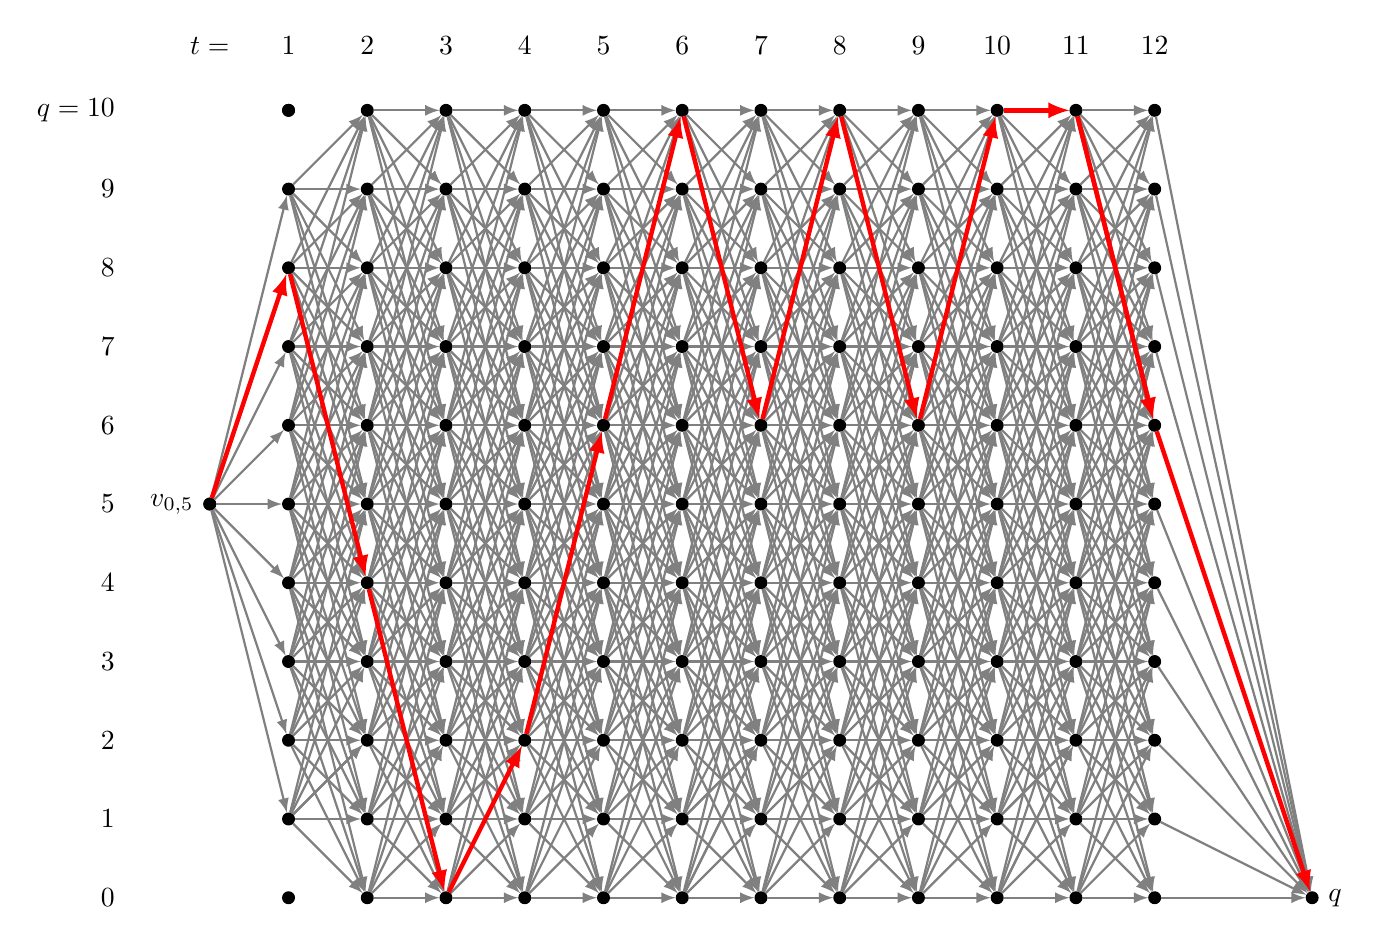
\begin{tikzpicture}

       \tikzset{enclosed/.style={draw, circle, inner sep=0pt, minimum size=.15cm, fill=black}}
%% Vertices
      	\node[enclosed, label={left: $v_{0,5}$}] (vstart) at (-1,5) {};
      	\node[enclosed, label={[label distance=5.5cm]90: $t=$}] (vstart) at (-1,5) {};
      	\node[enclosed, label={[label distance=2cm]180: $0$}] (v00) at (0,0) {};
    		\node[enclosed, label={[label distance=2cm]180: $1$}] (v01) at (0,1) {};
  	    \node[enclosed, label={[label distance=2cm]180: $2$}] (v02) at (0,2) {};
     	\node[enclosed, label={[label distance=2cm]180: $3$}] (v03) at (0,3) {};
     	\node[enclosed, label={[label distance=2cm]180: $4$}] (v04) at (0,4) {};
     	\node[enclosed, label={[label distance=2cm]180: $5$}] (v05) at (0,5) {};
     	\node[enclosed, label={[label distance=2cm]180: $6$}] (v06) at (0,6) {};
     	\node[enclosed, label={[label distance=2cm]180: $7$}] (v07) at (0,7) {};
     	\node[enclosed, label={[label distance=2cm]180: $8$}] (v08) at (0,8) {};
     	\node[enclosed, label={[label distance=2cm]180: $9$}] (v09) at (0,9) {};
     	\node[enclosed, label={[label distance=2cm]180: $q=10$}] (v010) at (0,10) {};
     	\node[enclosed, label={[label distance=0.5cm]90: $1$}] (v010) at (0,10) {};
      	\node[enclosed, label={above: }] (v10) at (1,0) {};
  	    \node[enclosed, label={below: }] (v11) at (1,1) {};
  	    \node[enclosed, label={below: }] (v12) at (1,2) {};
     	\node[enclosed, label={above:  }] (v13) at (1,3) {};
     	\node[enclosed, label={below: }] (v14) at (1,4) {};
     	 \node[enclosed, label={below:}] (v15) at (1,5) {};
     	\node[enclosed, label={above: }] (v16) at (1,6) {};
     	\node[enclosed, label={below: }] (v17) at (1,7) {};
     	\node[enclosed, label={above: }] (v18) at (1,8) {};
     	\node[enclosed, label={below:  }] (v19) at (1,9) {};
     	\node[enclosed, label={[label distance=0.5cm]90: $2$}] (v110) at (1,10) {};
     	\node[enclosed, label={below: }] (v20) at (2,0) {};
    		\node[enclosed, label={below: }] (v21) at (2,1) {};
  	    \node[enclosed, label={above: }] (v22) at (2,2) {};
     	\node[enclosed, label={below: }] (v23) at (2,3) {};
     	\node[enclosed, label={below:  }] (v24) at (2,4) {};
     	\node[enclosed, label={above: }] (v25) at (2,5) {};
     	\node[enclosed, label={below: }] (v26) at (2,6) {};
     	\node[enclosed, label={below: }] (v27) at (2,7) {};
     	\node[enclosed, label={above: }] (v28) at (2,8) {};
     	\node[enclosed, label={below:  }] (v29) at (2,9) {};
     	\node[enclosed, label={[label distance=0.5cm]90: $3$}] (v210) at (2,10) {};
      	\node[enclosed, label={above: }] (v30) at (3,0) {};
  	    \node[enclosed, label={below: }] (v31) at (3,1) {};
  	    \node[enclosed, label={below: }] (v32) at (3,2) {};
     	\node[enclosed, label={above:  }] (v33) at (3,3) {};
     	\node[enclosed, label={below: }] (v34) at (3,4) {};
     	 \node[enclosed, label={below:}] (v35) at (3,5) {};
     	\node[enclosed, label={above: }] (v36) at (3,6) {};
     	\node[enclosed, label={below: }] (v37) at (3,7) {};
     	\node[enclosed, label={above: }] (v38) at (3,8) {};
     	\node[enclosed, label={below:  }] (v39) at (3,9) {};
     	\node[enclosed, label={[label distance=0.5cm]90: $4$}] (v310) at (3,10) {};
     	 \node[enclosed, label={below: }] (v40) at (4,0) {};
    		\node[enclosed, label={below: }] (v41) at (4,1) {};
  	    \node[enclosed, label={above: }] (v42) at (4,2) {};
     	\node[enclosed, label={below: }] (v43) at (4,3) {};
     	\node[enclosed, label={below:  }] (v44) at (4,4) {};
     	\node[enclosed, label={above: }] (v45) at (4,5) {};
     	\node[enclosed, label={below: }] (v46) at (4,6) {};
     	\node[enclosed, label={below: }] (v47) at (4,7) {};
     	\node[enclosed, label={above: }] (v48) at (4,8) {};
     	\node[enclosed, label={below:  }] (v49) at (4,9) {};
     	\node[enclosed, label={[label distance=0.5cm]90: $5$}] (v410) at (4,10) {};
      	\node[enclosed, label={above: }] (v50) at (5,0) {};
  	    \node[enclosed, label={below: }] (v51) at (5,1) {};
  	    \node[enclosed, label={below: }] (v52) at (5,2) {};
     	\node[enclosed, label={above:  }] (v53) at (5,3) {};
     	\node[enclosed, label={below: }] (v54) at (5,4) {};
     	 \node[enclosed, label={below:}] (v55) at (5,5) {};
     	\node[enclosed, label={above: }] (v56) at (5,6) {};
     	\node[enclosed, label={below: }] (v57) at (5,7) {};
     	\node[enclosed, label={above: }] (v58) at (5,8) {};
     	\node[enclosed, label={below:  }] (v59) at (5,9) {};
     	\node[enclosed, label={[label distance=0.5cm]90: $6$}] (v510) at (5,10) {};
     	\node[enclosed, label={below: }] (v60) at (6,0) {};
    		\node[enclosed, label={below: }] (v61) at (6,1) {};
  	    \node[enclosed, label={above: }] (v62) at (6,2) {};
     	\node[enclosed, label={below: }] (v63) at (6,3) {};
     	\node[enclosed, label={below:  }] (v64) at (6,4) {};
     	\node[enclosed, label={above: }] (v65) at (6,5) {};
     	\node[enclosed, label={below: }] (v66) at (6,6) {};
     	\node[enclosed, label={below: }] (v67) at (6,7) {};
     	\node[enclosed, label={above: }] (v68) at (6,8) {};
     	\node[enclosed, label={below:  }] (v69) at (6,9) {};
     	\node[enclosed, label={[label distance=0.5cm]90: $7$}] (v610) at (6,10) {};
      	\node[enclosed, label={above: }] (v70) at (7,0) {};
  	    \node[enclosed, label={below: }] (v71) at (7,1) {};
  	    \node[enclosed, label={below: }] (v72) at (7,2) {};
     	\node[enclosed, label={above:  }] (v73) at (7,3) {};
     	\node[enclosed, label={below: }] (v74) at (7,4) {};
     	 \node[enclosed, label={below:}] (v75) at (7,5) {};
     	\node[enclosed, label={above: }] (v76) at (7,6) {};
     	\node[enclosed, label={below: }] (v77) at (7,7) {};
     	\node[enclosed, label={above: }] (v78) at (7,8) {};
     	\node[enclosed, label={below:  }] (v79) at (7,9) {};
     	\node[enclosed, label={[label distance=0.5cm]90: $8$}] (v710) at (7,10) {};
     	\node[enclosed, label={above: }] (v80) at (8,0) {};
  	    \node[enclosed, label={below: }] (v81) at (8,1) {};
  	    \node[enclosed, label={below: }] (v82) at (8,2) {};
     	\node[enclosed, label={above:  }] (v83) at (8,3) {};
     	\node[enclosed, label={below: }] (v84) at (8,4) {};
     	 \node[enclosed, label={below:}] (v85) at (8,5) {};
     	\node[enclosed, label={above: }] (v86) at (8,6) {};
     	\node[enclosed, label={below: }] (v87) at (8,7) {};
     	\node[enclosed, label={above: }] (v88) at (8,8) {};
     	\node[enclosed, label={below:  }] (v89) at (8,9) {};
     	\node[enclosed, label={[label distance=0.5cm]90: $9$}] (v810) at (8,10) {};
     	\node[enclosed, label={below: }] (v90) at (9,0) {};
    		\node[enclosed, label={below: }] (v91) at (9,1) {};
  	    \node[enclosed, label={above: }] (v92) at (9,2) {};
     	\node[enclosed, label={below: }] (v93) at (9,3) {};
     	\node[enclosed, label={below:  }] (v94) at (9,4) {};
     	\node[enclosed, label={above: }] (v95) at (9,5) {};
     	\node[enclosed, label={below: }] (v96) at (9,6) {};
     	\node[enclosed, label={below: }] (v97) at (9,7) {};
     	\node[enclosed, label={above: }] (v98) at (9,8) {};
     	\node[enclosed, label={below:  }] (v99) at (9,9) {};
     	\node[enclosed, label={[label distance=0.5cm]90: $10$}] (v910) at (9,10) {};
      	\node[enclosed, label={above: }] (v100) at (10,0) {};
  	    \node[enclosed, label={below: }] (v101) at (10,1) {};
  	    \node[enclosed, label={below: }] (v102) at (10,2) {};
     	\node[enclosed, label={above:  }] (v103) at (10,3) {};
     	\node[enclosed, label={below: }] (v104) at (10,4) {};
     	 \node[enclosed, label={below:}] (v105) at (10,5) {};
     	\node[enclosed, label={above: }] (v106) at (10,6) {};
     	\node[enclosed, label={below: }] (v107) at (10,7) {};
     	\node[enclosed, label={above: }] (v108) at (10,8) {};
     	\node[enclosed, label={below:  }] (v109) at (10,9) {};
     	\node[enclosed, label={[label distance=0.5cm]90: $11$}] (v1010) at (10,10) {};
     	\node[enclosed, label={above: }] (v1100) at (11,0) {};
  	    \node[enclosed, label={below: }] (v111) at (11,1) {};
  	    \node[enclosed, label={below: }] (v112) at (11,2) {};
     	\node[enclosed, label={above:  }] (v113) at (11,3) {};
     	\node[enclosed, label={below: }] (v114) at (11,4) {};
     	 \node[enclosed, label={below:}] (v115) at (11,5) {};
     	\node[enclosed, label={above: }] (v116) at (11,6) {};
     	\node[enclosed, label={below: }] (v117) at (11,7) {};
     	\node[enclosed, label={above: }] (v118) at (11,8) {};
     	\node[enclosed, label={below:  }] (v119) at (11,9) {};
     	\node[enclosed, label={[label distance=0.5cm]90: $12$}] (v1110) at (11,10) {};
     	\node[enclosed, label={right: $q_{\slut}$ }] (v120) at (13,0) {};
     	
%Edges
		\path[gray,->,>=latex,thick] (vstart) edge node[midway, sloped, above] {} (v01);
		\path[gray,->,>=latex,thick] (vstart) edge node[midway, sloped, below] {} (v02);
		\path[gray,->,>=latex,thick] (vstart) edge node[midway, sloped, below] {} (v03);
		\path[gray,->,>=latex,thick] (vstart) edge node[midway, sloped, above] {} (v04);
		\path[gray,->,>=latex,thick] (vstart) edge node[midway, above] {} (v05);
		\path[gray,->,>=latex,thick] (vstart) edge node[near end, sloped, below] {} (v06);
		\path[gray,->,>=latex,thick] (vstart) edge node[midway, sloped, below] {} (v07);
		\path[gray,->,>=latex,thick] (vstart) edge node[near end, sloped, below] {} (v09);
		\path[gray,->,>=latex,thick] (v01) edge node[midway, sloped, below] {} (v10);
		\path[gray,->,>=latex,thick] (v01) edge node[midway, sloped, above] {} (v11);
		\path[gray,->,>=latex,thick] (v01) edge node[midway, above] {} (v12);
		\path[gray,->,>=latex,thick] (v01) edge node[near end, sloped, below] {} (v12);
		\path[gray,->,>=latex,thick] (v01) edge node[midway, sloped, below] {} (v13);
		\path[gray,->,>=latex,thick] (v01) edge node[midway, above] {} (v14);
		\path[gray,->,>=latex,thick] (v01) edge node[near end, sloped, below] {} (v15);
		\path[gray,->,>=latex,thick] (v02) edge node[midway, sloped, below] {} (v10);
		\path[gray,->,>=latex,thick] (v02) edge node[midway, sloped, above] {} (v11);
		\path[gray,->,>=latex,thick] (v02) edge node[midway, above] {} (v12);
		\path[gray,->,>=latex,thick] (v02) edge node[near end, sloped, below] {} (v13);
		\path[gray,->,>=latex,thick] (v02) edge node[midway, sloped, below] {} (v14);
		\path[gray,->,>=latex,thick] (v02) edge node[midway, above] {} (v15);
		\path[gray,->,>=latex,thick] (v02) edge node[near end, sloped, below] {} (v16);
		\path[gray,->,>=latex,thick] (v03) edge node[midway, sloped, below] {} (v10);
		\path[gray,->,>=latex,thick] (v03) edge node[midway, sloped, above] {} (v11);
		\path[gray,->,>=latex,thick] (v03) edge node[midway, above] {} (v12);
		\path[gray,->,>=latex,thick] (v03) edge node[near end, sloped, below] {} (v13);
		\path[gray,->,>=latex,thick] (v03) edge node[midway, sloped, below] {} (v14);
		\path[gray,->,>=latex,thick] (v03) edge node[midway, above] {} (v15);
		\path[gray,->,>=latex,thick] (v03) edge node[near end, sloped, below] {} (v16);
		\path[gray,->,>=latex,thick] (v03) edge node[midway, sloped, below] {} (v17);
		\path[gray,->,>=latex,thick] (v04) edge node[midway, sloped, below] {} (v10);
		\path[gray,->,>=latex,thick] (v04) edge node[midway, sloped, above] {} (v11);
		\path[gray,->,>=latex,thick] (v04) edge node[midway, above] {} (v12);
		\path[gray,->,>=latex,thick] (v04) edge node[near end, sloped, below] {} (v13);
		\path[gray,->,>=latex,thick] (v04) edge node[midway, sloped, below] {} (v14);
		\path[gray,->,>=latex,thick] (v04) edge node[midway, above] {} (v15);
		\path[gray,->,>=latex,thick] (v04) edge node[near end, sloped, below] {} (v16);
		\path[gray,->,>=latex,thick] (v04) edge node[midway, sloped, below] {} (v17);
		\path[gray,->,>=latex,thick] (v04) edge node[midway, sloped, above] {} (v18);
		\path[gray,->,>=latex,thick] (v05) edge node[midway, sloped, above] {} (v11);
		\path[gray,->,>=latex,thick] (v05) edge node[midway, above] {} (v12);
		\path[gray,->,>=latex,thick] (v05) edge node[near end, sloped, below] {} (v13);
		\path[gray,->,>=latex,thick] (v05) edge node[midway, sloped, below] {} (v14);
		\path[gray,->,>=latex,thick] (v05) edge node[midway, above] {} (v15);
		\path[gray,->,>=latex,thick] (v05) edge node[near end, sloped, below] {} (v16);
		\path[gray,->,>=latex,thick] (v05) edge node[midway, sloped, below] {} (v17);
		\path[gray,->,>=latex,thick] (v05) edge node[midway, sloped, above] {} (v18);
		\path[gray,->,>=latex,thick] (v05) edge node[midway, sloped, above] {} (v19);
		\path[gray,->,>=latex,thick] (v06) edge node[midway, above] {} (v12);
		\path[gray,->,>=latex,thick] (v06) edge node[near end, sloped, below] {} (v13);
		\path[gray,->,>=latex,thick] (v06) edge node[midway, sloped, below] {} (v14);
		\path[gray,->,>=latex,thick] (v06) edge node[midway, above] {} (v15);
		\path[gray,->,>=latex,thick] (v06) edge node[near end, sloped, below] {} (v16);
		\path[gray,->,>=latex,thick] (v06) edge node[midway, sloped, below] {} (v17);
		\path[gray,->,>=latex,thick] (v06) edge node[midway, sloped, above] {} (v18);
		\path[gray,->,>=latex,thick] (v06) edge node[midway, sloped, above] {} (v19);
		\path[gray,->,>=latex,thick] (v06) edge node[midway, sloped, above] {} (v110);
		\path[gray,->,>=latex,thick] (v07) edge node[near end, sloped, below] {} (v13);
		\path[gray,->,>=latex,thick] (v07) edge node[midway, sloped, below] {} (v14);
		\path[gray,->,>=latex,thick] (v07) edge node[midway, above] {} (v15);
		\path[gray,->,>=latex,thick] (v07) edge node[near end, sloped, below] {} (v16);
		\path[gray,->,>=latex,thick] (v07) edge node[midway, sloped, below] {} (v17);
		\path[gray,->,>=latex,thick] (v07) edge node[midway, sloped, above] {} (v18);
		\path[gray,->,>=latex,thick] (v07) edge node[midway, sloped, above] {} (v19);
		\path[gray,->,>=latex,thick] (v07) edge node[midway, sloped, above] {} (v110);
		\path[gray,->,>=latex,thick] (v08) edge node[midway, above] {} (v15);
		\path[gray,->,>=latex,thick] (v08) edge node[near end, sloped, below] {} (v16);
		\path[gray,->,>=latex,thick] (v08) edge node[midway, sloped, below] {} (v17);
		\path[gray,->,>=latex,thick] (v08) edge node[midway, sloped, above] {} (v18);
		\path[gray,->,>=latex,thick] (v08) edge node[midway, sloped, above] {} (v19);
		\path[gray,->,>=latex,thick] (v08) edge node[midway, sloped, above] {} (v110);
		\path[gray,->,>=latex,thick] (v09) edge node[midway, above] {} (v15);
		\path[gray,->,>=latex,thick] (v09) edge node[near end, sloped, below] {} (v16);
		\path[gray,->,>=latex,thick] (v09) edge node[midway, sloped, below] {} (v17);
		\path[gray,->,>=latex,thick] (v09) edge node[midway, sloped, above] {} (v18);
		\path[gray,->,>=latex,thick] (v09) edge node[midway, sloped, above] {} (v19);
		\path[gray,->,>=latex,thick] (v09) edge node[midway, sloped, above] {} (v110);
		\path[gray,->,>=latex,thick] (v10) edge node[midway, sloped, below] {} (v20);
		\path[gray,->,>=latex,thick] (v10) edge node[midway, sloped, above] {} (v21);
		\path[gray,->,>=latex,thick] (v10) edge node[midway, above] {} (v22);
		\path[gray,->,>=latex,thick] (v10) edge node[midway, sloped, below] {} (v23);
		\path[gray,->,>=latex,thick] (v10) edge node[midway, above] {} (v24);
		\path[gray,->,>=latex,thick] (v11) edge node[midway, sloped, below] {} (v20);
		\path[gray,->,>=latex,thick] (v11) edge node[midway, sloped, above] {} (v21);
		\path[gray,->,>=latex,thick] (v11) edge node[midway, above] {} (v22);
		\path[gray,->,>=latex,thick] (v11) edge node[midway, sloped, below] {} (v23);
		\path[gray,->,>=latex,thick] (v11) edge node[midway, above] {} (v24);
		\path[gray,->,>=latex,thick] (v11) edge node[near end, sloped, below] {} (v25);
		\path[gray,->,>=latex,thick] (v12) edge node[midway, sloped, below] {} (v20);
		\path[gray,->,>=latex,thick] (v12) edge node[midway, sloped, above] {} (v21);
		\path[gray,->,>=latex,thick] (v12) edge node[midway, above] {} (v22);
		\path[gray,->,>=latex,thick] (v12) edge node[near end, sloped, below] {} (v23);
		\path[gray,->,>=latex,thick] (v12) edge node[midway, sloped, below] {} (v24);
		\path[gray,->,>=latex,thick] (v12) edge node[midway, above] {} (v25);
		\path[gray,->,>=latex,thick] (v12) edge node[near end, sloped, below] {} (v26);
		\path[gray,->,>=latex,thick] (v13) edge node[midway, sloped, below] {} (v20);
		\path[gray,->,>=latex,thick] (v13) edge node[midway, sloped, above] {} (v21);
		\path[gray,->,>=latex,thick] (v13) edge node[midway, above] {} (v22);
		\path[gray,->,>=latex,thick] (v13) edge node[near end, sloped, below] {} (v23);
		\path[gray,->,>=latex,thick] (v13) edge node[midway, sloped, below] {} (v24);
		\path[gray,->,>=latex,thick] (v13) edge node[midway, above] {} (v25);
		\path[gray,->,>=latex,thick] (v13) edge node[near end, sloped, below] {} (v26);
		\path[gray,->,>=latex,thick] (v13) edge node[midway, sloped, below] {} (v27);
		\path[gray,->,>=latex,thick] (v14) edge node[midway, sloped, above] {} (v21);
		\path[gray,->,>=latex,thick] (v14) edge node[midway, above] {} (v22);
		\path[gray,->,>=latex,thick] (v14) edge node[near end, sloped, below] {} (v23);
		\path[gray,->,>=latex,thick] (v14) edge node[midway, sloped, below] {} (v24);
		\path[gray,->,>=latex,thick] (v14) edge node[midway, above] {} (v25);
		\path[gray,->,>=latex,thick] (v14) edge node[near end, sloped, below] {} (v26);
		\path[gray,->,>=latex,thick] (v14) edge node[midway, sloped, below] {} (v27);
		\path[gray,->,>=latex,thick] (v14) edge node[midway, sloped, above] {} (v28);
		\path[gray,->,>=latex,thick] (v15) edge node[midway, sloped, above] {} (v21);
		\path[gray,->,>=latex,thick] (v15) edge node[midway, above] {} (v22);
		\path[gray,->,>=latex,thick] (v15) edge node[near end, sloped, below] {} (v23);
		\path[gray,->,>=latex,thick] (v15) edge node[midway, sloped, below] {} (v24);
		\path[gray,->,>=latex,thick] (v15) edge node[midway, above] {} (v25);
		\path[gray,->,>=latex,thick] (v15) edge node[near end, sloped, below] {} (v26);
		\path[gray,->,>=latex,thick] (v15) edge node[midway, sloped, below] {} (v27);
		\path[gray,->,>=latex,thick] (v15) edge node[midway, sloped, above] {} (v28);
		\path[gray,->,>=latex,thick] (v15) edge node[midway, sloped, above] {} (v29);
		\path[gray,->,>=latex,thick] (v16) edge node[midway, above] {} (v22);
		\path[gray,->,>=latex,thick] (v16) edge node[near end, sloped, below] {} (v23);
		\path[gray,->,>=latex,thick] (v16) edge node[midway, sloped, below] {} (v24);
		\path[gray,->,>=latex,thick] (v16) edge node[midway, above] {} (v25);
		\path[gray,->,>=latex,thick] (v16) edge node[near end, sloped, below] {} (v26);
		\path[gray,->,>=latex,thick] (v16) edge node[midway, sloped, below] {} (v27);
		\path[gray,->,>=latex,thick] (v16) edge node[midway, sloped, above] {} (v28);
		\path[gray,->,>=latex,thick] (v16) edge node[midway, sloped, above] {} (v29);
		\path[gray,->,>=latex,thick] (v16) edge node[midway, sloped, above] {} (v210);
		\path[gray,->,>=latex,thick] (v17) edge node[near end, sloped, below] {} (v23);
		\path[gray,->,>=latex,thick] (v17) edge node[midway, sloped, below] {} (v24);
		\path[gray,->,>=latex,thick] (v17) edge node[midway, above] {} (v25);
		\path[gray,->,>=latex,thick] (v17) edge node[near end, sloped, below] {} (v26);
		\path[gray,->,>=latex,thick] (v17) edge node[midway, sloped, below] {} (v27);
		\path[gray,->,>=latex,thick] (v17) edge node[midway, sloped, above] {} (v28);
		\path[gray,->,>=latex,thick] (v17) edge node[midway, sloped, above] {} (v29);
		\path[gray,->,>=latex,thick] (v17) edge node[midway, sloped, above] {} (v210);
		\path[gray,->,>=latex,thick] (v18) edge node[midway, sloped, below] {} (v24);
		\path[gray,->,>=latex,thick] (v18) edge node[midway, above] {} (v25);
		\path[gray,->,>=latex,thick] (v18) edge node[near end, sloped, below] {} (v26);
		\path[gray,->,>=latex,thick] (v18) edge node[midway, sloped, below] {} (v27);
		\path[gray,->,>=latex,thick] (v18) edge node[midway, sloped, above] {} (v28);
		\path[gray,->,>=latex,thick] (v18) edge node[midway, sloped, above] {} (v29);
		\path[gray,->,>=latex,thick] (v18) edge node[midway, sloped, above] {} (v210);
		\path[gray,->,>=latex,thick] (v19) edge node[midway, above] {} (v25);
		\path[gray,->,>=latex,thick] (v19) edge node[near end, sloped, below] {} (v26);
		\path[gray,->,>=latex,thick] (v19) edge node[midway, sloped, below] {} (v27);
		\path[gray,->,>=latex,thick] (v19) edge node[midway, sloped, above] {} (v28);
		\path[gray,->,>=latex,thick] (v19) edge node[midway, sloped, above] {} (v29);
		\path[gray,->,>=latex,thick] (v19) edge node[midway, sloped, above] {} (v210);
		\path[gray,->,>=latex,thick] (v110) edge node[near end, sloped, below] {} (v26);
		\path[gray,->,>=latex,thick] (v110) edge node[midway, sloped, below] {} (v27);
		\path[gray,->,>=latex,thick] (v110) edge node[midway, sloped, above] {} (v28);
		\path[gray,->,>=latex,thick] (v110) edge node[midway, sloped, above] {} (v29);
		\path[gray,->,>=latex,thick] (v110) edge node[midway, sloped, above] {} (v210);
		\path[gray,->,>=latex,thick] (v20) edge node[midway, sloped, below] {} (v30);
		\path[gray,->,>=latex,thick] (v20) edge node[midway, sloped, above] {} (v31);
		\path[gray,->,>=latex,thick] (v20) edge node[near end, sloped, below] {} (v32);
		\path[gray,->,>=latex,thick] (v20) edge node[midway, sloped, below] {} (v33);
		\path[gray,->,>=latex,thick] (v20) edge node[midway, above] {} (v34);
		\path[gray,->,>=latex,thick] (v21) edge node[midway, sloped, below] {} (v30);
		\path[gray,->,>=latex,thick] (v21) edge node[midway, sloped, above] {} (v31);
		\path[gray,->,>=latex,thick] (v21) edge node[midway, above] {} (v32);
		\path[gray,->,>=latex,thick] (v21) edge node[near end, sloped, below] {} (v32);
		\path[gray,->,>=latex,thick] (v21) edge node[midway, sloped, below] {} (v33);
		\path[gray,->,>=latex,thick] (v21) edge node[midway, above] {} (v34);
		\path[gray,->,>=latex,thick] (v21) edge node[near end, sloped, below] {} (v35);
		\path[gray,->,>=latex,thick] (v22) edge node[midway, sloped, below] {} (v30);
		\path[gray,->,>=latex,thick] (v22) edge node[midway, sloped, above] {} (v31);
		\path[gray,->,>=latex,thick] (v22) edge node[midway, above] {} (v32);
		\path[gray,->,>=latex,thick] (v22) edge node[near end, sloped, below] {} (v33);
		\path[gray,->,>=latex,thick] (v22) edge node[midway, sloped, below] {} (v34);
		\path[gray,->,>=latex,thick] (v22) edge node[midway, above] {} (v35);
		\path[gray,->,>=latex,thick] (v22) edge node[near end, sloped, below] {} (v36);
		\path[gray,->,>=latex,thick] (v23) edge node[midway, sloped, below] {} (v30);
		\path[gray,->,>=latex,thick] (v23) edge node[midway, sloped, above] {} (v31);
		\path[gray,->,>=latex,thick] (v23) edge node[midway, above] {} (v32);
		\path[gray,->,>=latex,thick] (v23) edge node[near end, sloped, below] {} (v33);
		\path[gray,->,>=latex,thick] (v23) edge node[midway, sloped, below] {} (v34);
		\path[gray,->,>=latex,thick] (v23) edge node[midway, above] {} (v35);
		\path[gray,->,>=latex,thick] (v23) edge node[near end, sloped, below] {} (v36);
		\path[gray,->,>=latex,thick] (v23) edge node[midway, sloped, below] {} (v37);
		\path[gray,->,>=latex,thick] (v24) edge node[midway, sloped, below] {} (v30);
		\path[gray,->,>=latex,thick] (v24) edge node[midway, sloped, above] {} (v31);
		\path[gray,->,>=latex,thick] (v24) edge node[midway, above] {} (v32);
		\path[gray,->,>=latex,thick] (v24) edge node[near end, sloped, below] {} (v33);
		\path[gray,->,>=latex,thick] (v24) edge node[midway, sloped, below] {} (v34);
		\path[gray,->,>=latex,thick] (v24) edge node[midway, above] {} (v35);
		\path[gray,->,>=latex,thick] (v24) edge node[near end, sloped, below] {} (v36);
		\path[gray,->,>=latex,thick] (v24) edge node[midway, sloped, below] {} (v37);
		\path[gray,->,>=latex,thick] (v24) edge node[midway, sloped, above] {} (v38);
		\path[gray,->,>=latex,thick] (v25) edge node[midway, sloped, above] {} (v31);
		\path[gray,->,>=latex,thick] (v25) edge node[midway, above] {} (v32);
		\path[gray,->,>=latex,thick] (v25) edge node[near end, sloped, below] {} (v33);
		\path[gray,->,>=latex,thick] (v25) edge node[midway, sloped, below] {} (v34);
		\path[gray,->,>=latex,thick] (v25) edge node[midway, above] {} (v35);
		\path[gray,->,>=latex,thick] (v25) edge node[near end, sloped, below] {} (v36);
		\path[gray,->,>=latex,thick] (v25) edge node[midway, sloped, below] {} (v37);
		\path[gray,->,>=latex,thick] (v25) edge node[midway, sloped, above] {} (v38);
		\path[gray,->,>=latex,thick] (v25) edge node[midway, sloped, above] {} (v39);
		\path[gray,->,>=latex,thick] (v26) edge node[midway, above] {} (v32);
		\path[gray,->,>=latex,thick] (v26) edge node[near end, sloped, below] {} (v33);
		\path[gray,->,>=latex,thick] (v26) edge node[midway, sloped, below] {} (v34);
		\path[gray,->,>=latex,thick] (v26) edge node[midway, above] {} (v35);
		\path[gray,->,>=latex,thick] (v26) edge node[near end, sloped, below] {} (v36);
		\path[gray,->,>=latex,thick] (v26) edge node[midway, sloped, below] {} (v37);
		\path[gray,->,>=latex,thick] (v26) edge node[midway, sloped, above] {} (v38);
		\path[gray,->,>=latex,thick] (v26) edge node[midway, sloped, above] {} (v39);
		\path[gray,->,>=latex,thick] (v26) edge node[midway, sloped, above] {} (v310);
		\path[gray,->,>=latex,thick] (v27) edge node[near end, sloped, below] {} (v33);
		\path[gray,->,>=latex,thick] (v27) edge node[midway, sloped, below] {} (v34);
		\path[gray,->,>=latex,thick] (v27) edge node[midway, above] {} (v35);
		\path[gray,->,>=latex,thick] (v27) edge node[near end, sloped, below] {} (v36);
		\path[gray,->,>=latex,thick] (v27) edge node[midway, sloped, below] {} (v37);
		\path[gray,->,>=latex,thick] (v27) edge node[midway, sloped, above] {} (v38);
		\path[gray,->,>=latex,thick] (v27) edge node[midway, sloped, above] {} (v39);
		\path[gray,->,>=latex,thick] (v27) edge node[midway, sloped, above] {} (v310);
		\path[gray,->,>=latex,thick] (v28) edge node[midway, sloped, below] {} (v34);
		\path[gray,->,>=latex,thick] (v28) edge node[midway, above] {} (v35);
		\path[gray,->,>=latex,thick] (v28) edge node[near end, sloped, below] {} (v36);
		\path[gray,->,>=latex,thick] (v28) edge node[midway, sloped, below] {} (v37);
		\path[gray,->,>=latex,thick] (v28) edge node[midway, sloped, above] {} (v38);
		\path[gray,->,>=latex,thick] (v28) edge node[midway, sloped, above] {} (v39);
		\path[gray,->,>=latex,thick] (v28) edge node[midway, sloped, above] {} (v310);
		\path[gray,->,>=latex,thick] (v29) edge node[midway, above] {} (v35);
		\path[gray,->,>=latex,thick] (v29) edge node[near end, sloped, below] {} (v36);
		\path[gray,->,>=latex,thick] (v29) edge node[midway, sloped, below] {} (v37);
		\path[gray,->,>=latex,thick] (v29) edge node[midway, sloped, above] {} (v38);
		\path[gray,->,>=latex,thick] (v29) edge node[midway, sloped, above] {} (v39);
		\path[gray,->,>=latex,thick] (v29) edge node[midway, sloped, above] {} (v310);
		\path[gray,->,>=latex,thick] (v210) edge node[near end, sloped, below] {} (v36);
		\path[gray,->,>=latex,thick] (v210) edge node[midway, sloped, below] {} (v37);
		\path[gray,->,>=latex,thick] (v210) edge node[midway, sloped, above] {} (v38);
		\path[gray,->,>=latex,thick] (v210) edge node[midway, sloped, above] {} (v39);
		\path[gray,->,>=latex,thick] (v210) edge node[midway, sloped, above] {} (v310);
		\path[gray,->,>=latex,thick] (v30) edge node[midway, sloped, below] {} (v40);
		\path[gray,->,>=latex,thick] (v30) edge node[midway, sloped, above] {} (v41);
		\path[gray,->,>=latex,thick] (v30) edge node[midway, above] {} (v42);
		\path[gray,->,>=latex,thick] (v30) edge node[midway, sloped, below] {} (v43);
		\path[gray,->,>=latex,thick] (v30) edge node[midway, above] {} (v44);
		\path[gray,->,>=latex,thick] (v31) edge node[midway, sloped, below] {} (v40);
		\path[gray,->,>=latex,thick] (v31) edge node[midway, sloped, above] {} (v41);
		\path[gray,->,>=latex,thick] (v31) edge node[midway, above] {} (v42);
		\path[gray,->,>=latex,thick] (v31) edge node[midway, sloped, below] {} (v43);
		\path[gray,->,>=latex,thick] (v31) edge node[midway, above] {} (v44);
		\path[gray,->,>=latex,thick] (v31) edge node[near end, sloped, below] {} (v45);
		\path[gray,->,>=latex,thick] (v32) edge node[midway, sloped, below] {} (v40);
		\path[gray,->,>=latex,thick] (v32) edge node[midway, sloped, above] {} (v41);
		\path[gray,->,>=latex,thick] (v32) edge node[midway, above] {} (v42);
		\path[gray,->,>=latex,thick] (v32) edge node[near end, sloped, below] {} (v43);
		\path[gray,->,>=latex,thick] (v32) edge node[midway, sloped, below] {} (v44);
		\path[gray,->,>=latex,thick] (v32) edge node[midway, above] {} (v45);
		\path[gray,->,>=latex,thick] (v33) edge node[midway, sloped, below] {} (v40);
		\path[gray,->,>=latex,thick] (v33) edge node[midway, sloped, above] {} (v41);
		\path[gray,->,>=latex,thick] (v33) edge node[midway, above] {} (v42);
		\path[gray,->,>=latex,thick] (v33) edge node[near end, sloped, below] {} (v43);
		\path[gray,->,>=latex,thick] (v33) edge node[midway, sloped, below] {} (v44);
		\path[gray,->,>=latex,thick] (v33) edge node[midway, above] {} (v45);
		\path[gray,->,>=latex,thick] (v33) edge node[near end, sloped, below] {} (v46);
		\path[gray,->,>=latex,thick] (v33) edge node[midway, sloped, below] {} (v47);
		\path[gray,->,>=latex,thick] (v34) edge node[midway, sloped, below] {} (v40);
		\path[gray,->,>=latex,thick] (v34) edge node[midway, sloped, above] {} (v41);
		\path[gray,->,>=latex,thick] (v34) edge node[midway, above] {} (v42);
		\path[gray,->,>=latex,thick] (v34) edge node[near end, sloped, below] {} (v43);
		\path[gray,->,>=latex,thick] (v34) edge node[midway, sloped, below] {} (v44);
		\path[gray,->,>=latex,thick] (v34) edge node[midway, above] {} (v45);
		\path[gray,->,>=latex,thick] (v34) edge node[near end, sloped, below] {} (v46);
		\path[gray,->,>=latex,thick] (v34) edge node[midway, sloped, below] {} (v47);
		\path[gray,->,>=latex,thick] (v34) edge node[midway, sloped, above] {} (v48);
		\path[gray,->,>=latex,thick] (v35) edge node[midway, sloped, above] {} (v41);
		\path[gray,->,>=latex,thick] (v35) edge node[midway, above] {} (v42);
		\path[gray,->,>=latex,thick] (v35) edge node[near end, sloped, below] {} (v43);
		\path[gray,->,>=latex,thick] (v35) edge node[midway, sloped, below] {} (v44);
		\path[gray,->,>=latex,thick] (v35) edge node[midway, above] {} (v45);
		\path[gray,->,>=latex,thick] (v35) edge node[near end, sloped, below] {} (v46);
		\path[gray,->,>=latex,thick] (v35) edge node[midway, sloped, below] {} (v47);
		\path[gray,->,>=latex,thick] (v35) edge node[midway, sloped, above] {} (v48);
		\path[gray,->,>=latex,thick] (v35) edge node[midway, sloped, above] {} (v49);
		\path[gray,->,>=latex,thick] (v36) edge node[midway, above] {} (v42);
		\path[gray,->,>=latex,thick] (v36) edge node[near end, sloped, below] {} (v43);
		\path[gray,->,>=latex,thick] (v36) edge node[midway, sloped, below] {} (v44);
		\path[gray,->,>=latex,thick] (v36) edge node[midway, above] {} (v45);
		\path[gray,->,>=latex,thick] (v36) edge node[near end, sloped, below] {} (v46);
		\path[gray,->,>=latex,thick] (v36) edge node[midway, sloped, below] {} (v47);
		\path[gray,->,>=latex,thick] (v36) edge node[midway, sloped, above] {} (v48);
		\path[gray,->,>=latex,thick] (v36) edge node[midway, sloped, above] {} (v49);
		\path[gray,->,>=latex,thick] (v36) edge node[midway, sloped, above] {} (v410);
		\path[gray,->,>=latex,thick] (v37) edge node[near end, sloped, below] {} (v43);
		\path[gray,->,>=latex,thick] (v37) edge node[midway, sloped, below] {} (v44);
		\path[gray,->,>=latex,thick] (v37) edge node[midway, above] {} (v45);
		\path[gray,->,>=latex,thick] (v37) edge node[near end, sloped, below] {} (v46);
		\path[gray,->,>=latex,thick] (v37) edge node[midway, sloped, below] {} (v47);
		\path[gray,->,>=latex,thick] (v37) edge node[midway, sloped, above] {} (v48);
		\path[gray,->,>=latex,thick] (v37) edge node[midway, sloped, above] {} (v49);
		\path[gray,->,>=latex,thick] (v37) edge node[midway, sloped, above] {} (v410);
		\path[gray,->,>=latex,thick] (v38) edge node[midway, sloped, below] {} (v44);
		\path[gray,->,>=latex,thick] (v38) edge node[midway, above] {} (v45);
		\path[gray,->,>=latex,thick] (v38) edge node[near end, sloped, below] {} (v46);
		\path[gray,->,>=latex,thick] (v38) edge node[midway, sloped, below] {} (v47);
		\path[gray,->,>=latex,thick] (v38) edge node[midway, sloped, above] {} (v48);
		\path[gray,->,>=latex,thick] (v38) edge node[midway, sloped, above] {} (v49);
		\path[gray,->,>=latex,thick] (v38) edge node[midway, sloped, above] {} (v410);
		\path[gray,->,>=latex,thick] (v39) edge node[midway, above] {} (v45);
		\path[gray,->,>=latex,thick] (v39) edge node[near end, sloped, below] {} (v46);
		\path[gray,->,>=latex,thick] (v39) edge node[midway, sloped, below] {} (v47);
		\path[gray,->,>=latex,thick] (v39) edge node[midway, sloped, above] {} (v48);
		\path[gray,->,>=latex,thick] (v39) edge node[midway, sloped, above] {} (v49);
		\path[gray,->,>=latex,thick] (v39) edge node[midway, sloped, above] {} (v410);
		\path[gray,->,>=latex,thick] (v310) edge node[near end, sloped, below] {} (v46);
		\path[gray,->,>=latex,thick] (v310) edge node[midway, sloped, below] {} (v47);
		\path[gray,->,>=latex,thick] (v310) edge node[midway, sloped, above] {} (v48);
		\path[gray,->,>=latex,thick] (v310) edge node[midway, sloped, above] {} (v49);
		\path[gray,->,>=latex,thick] (v310) edge node[midway, sloped, above] {} (v410);
		\path[gray,->,>=latex,thick] (v40) edge node[midway, sloped, below] {} (v50);
		\path[gray,->,>=latex,thick] (v40) edge node[midway, sloped, above] {} (v51);
		\path[gray,->,>=latex,thick] (v40) edge node[midway, above] {} (v52);
		\path[gray,->,>=latex,thick] (v40) edge node[midway, sloped, below] {} (v53);
		\path[gray,->,>=latex,thick] (v40) edge node[midway, above] {} (v54);
		\path[gray,->,>=latex,thick] (v41) edge node[midway, sloped, below] {} (v50);
		\path[gray,->,>=latex,thick] (v41) edge node[midway, sloped, above] {} (v51);
		\path[gray,->,>=latex,thick] (v41) edge node[midway, above] {} (v52);
		\path[gray,->,>=latex,thick] (v41) edge node[midway, sloped, below] {} (v53);
		\path[gray,->,>=latex,thick] (v41) edge node[midway, above] {} (v54);
		\path[gray,->,>=latex,thick] (v41) edge node[near end, sloped, below] {} (v55);
		\path[gray,->,>=latex,thick] (v42) edge node[midway, sloped, below] {} (v50);
		\path[gray,->,>=latex,thick] (v42) edge node[midway, sloped, above] {} (v51);
		\path[gray,->,>=latex,thick] (v42) edge node[midway, above] {} (v52);
		\path[gray,->,>=latex,thick] (v42) edge node[near end, sloped, below] {} (v53);
		\path[gray,->,>=latex,thick] (v42) edge node[midway, sloped, below] {} (v54);
		\path[gray,->,>=latex,thick] (v42) edge node[midway, above] {} (v55);
		\path[gray,->,>=latex,thick] (v42) edge node[near end, sloped, below] {} (v56);
		\path[gray,->,>=latex,thick] (v43) edge node[midway, sloped, below] {} (v50);
		\path[gray,->,>=latex,thick] (v43) edge node[midway, sloped, above] {} (v51);
		\path[gray,->,>=latex,thick] (v43) edge node[midway, above] {} (v52);
		\path[gray,->,>=latex,thick] (v43) edge node[near end, sloped, below] {} (v53);
		\path[gray,->,>=latex,thick] (v43) edge node[midway, sloped, below] {} (v54);
		\path[gray,->,>=latex,thick] (v43) edge node[midway, above] {} (v55);
		\path[gray,->,>=latex,thick] (v43) edge node[near end, sloped, below] {} (v56);
		\path[gray,->,>=latex,thick] (v43) edge node[midway, sloped, below] {} (v57);
		\path[gray,->,>=latex,thick] (v44) edge node[midway, sloped, below] {} (v50);
		\path[gray,->,>=latex,thick] (v44) edge node[midway, sloped, above] {} (v51);
		\path[gray,->,>=latex,thick] (v44) edge node[midway, above] {} (v52);
		\path[gray,->,>=latex,thick] (v44) edge node[near end, sloped, below] {} (v53);
		\path[gray,->,>=latex,thick] (v44) edge node[midway, sloped, below] {} (v54);
		\path[gray,->,>=latex,thick] (v44) edge node[midway, above] {} (v55);
		\path[gray,->,>=latex,thick] (v44) edge node[near end, sloped, below] {} (v56);
		\path[gray,->,>=latex,thick] (v44) edge node[midway, sloped, below] {} (v57);
		\path[gray,->,>=latex,thick] (v44) edge node[midway, sloped, above] {} (v58);
		\path[gray,->,>=latex,thick] (v45) edge node[midway, sloped, above] {} (v51);
		\path[gray,->,>=latex,thick] (v45) edge node[midway, above] {} (v52);
		\path[gray,->,>=latex,thick] (v45) edge node[near end, sloped, below] {} (v53);
		\path[gray,->,>=latex,thick] (v45) edge node[midway, sloped, below] {} (v54);
		\path[gray,->,>=latex,thick] (v45) edge node[midway, above] {} (v55);
		\path[gray,->,>=latex,thick] (v45) edge node[near end, sloped, below] {} (v56);
		\path[gray,->,>=latex,thick] (v45) edge node[midway, sloped, below] {} (v57);
		\path[gray,->,>=latex,thick] (v45) edge node[midway, sloped, above] {} (v58);
		\path[gray,->,>=latex,thick] (v45) edge node[midway, sloped, above] {} (v59);
		\path[gray,->,>=latex,thick] (v46) edge node[midway, above] {} (v52);
		\path[gray,->,>=latex,thick] (v46) edge node[near end, sloped, below] {} (v53);
		\path[gray,->,>=latex,thick] (v46) edge node[midway, sloped, below] {} (v54);
		\path[gray,->,>=latex,thick] (v46) edge node[midway, above] {} (v55);
		\path[gray,->,>=latex,thick] (v46) edge node[near end, sloped, below] {} (v56);
		\path[gray,->,>=latex,thick] (v46) edge node[midway, sloped, below] {} (v57);
		\path[gray,->,>=latex,thick] (v46) edge node[midway, sloped, above] {} (v58);
		\path[gray,->,>=latex,thick] (v46) edge node[midway, sloped, above] {} (v59);
		\path[gray,->,>=latex,thick] (v47) edge node[near end, sloped, below] {} (v53);
		\path[gray,->,>=latex,thick] (v47) edge node[midway, sloped, below] {} (v54);
		\path[gray,->,>=latex,thick] (v47) edge node[midway, above] {} (v55);
		\path[gray,->,>=latex,thick] (v47) edge node[near end, sloped, below] {} (v56);
		\path[gray,->,>=latex,thick] (v47) edge node[midway, sloped, below] {} (v57);
		\path[gray,->,>=latex,thick] (v47) edge node[midway, sloped, above] {} (v58);
		\path[gray,->,>=latex,thick] (v47) edge node[midway, sloped, above] {} (v59);
		\path[gray,->,>=latex,thick] (v47) edge node[midway, sloped, above] {} (v510);
		\path[gray,->,>=latex,thick] (v48) edge node[midway, sloped, below] {} (v54);
		\path[gray,->,>=latex,thick] (v48) edge node[midway, above] {} (v55);
		\path[gray,->,>=latex,thick] (v48) edge node[near end, sloped, below] {} (v56);
		\path[gray,->,>=latex,thick] (v48) edge node[midway, sloped, below] {} (v57);
		\path[gray,->,>=latex,thick] (v48) edge node[midway, sloped, above] {} (v58);
		\path[gray,->,>=latex,thick] (v48) edge node[midway, sloped, above] {} (v59);
		\path[gray,->,>=latex,thick] (v48) edge node[midway, sloped, above] {} (v510);
		\path[gray,->,>=latex,thick] (v49) edge node[midway, above] {} (v55);
		\path[gray,->,>=latex,thick] (v49) edge node[near end, sloped, below] {} (v56);
		\path[gray,->,>=latex,thick] (v49) edge node[midway, sloped, below] {} (v57);
		\path[gray,->,>=latex,thick] (v49) edge node[midway, sloped, above] {} (v58);
		\path[gray,->,>=latex,thick] (v49) edge node[midway, sloped, above] {} (v59);
		\path[gray,->,>=latex,thick] (v49) edge node[midway, sloped, above] {} (v510);
		\path[gray,->,>=latex,thick] (v410) edge node[near end, sloped, below] {} (v56);
		\path[gray,->,>=latex,thick] (v410) edge node[midway, sloped, below] {} (v57);
		\path[gray,->,>=latex,thick] (v410) edge node[midway, sloped, above] {} (v58);
		\path[gray,->,>=latex,thick] (v410) edge node[midway, sloped, above] {} (v59);
		\path[gray,->,>=latex,thick] (v410) edge node[midway, sloped, above] {} (v510);
		\path[gray,->,>=latex,thick] (v50) edge node[midway, sloped, below] {} (v60);
		\path[gray,->,>=latex,thick] (v50) edge node[midway, sloped, above] {} (v61);
		\path[gray,->,>=latex,thick] (v50) edge node[midway, above] {} (v62);
		\path[gray,->,>=latex,thick] (v50) edge node[near end, sloped, below] {} (v62);
		\path[gray,->,>=latex,thick] (v50) edge node[midway, sloped, below] {} (v63);
		\path[gray,->,>=latex,thick] (v50) edge node[midway, above] {} (v64);
		\path[gray,->,>=latex,thick] (v51) edge node[midway, sloped, below] {} (v60);
		\path[gray,->,>=latex,thick] (v51) edge node[midway, sloped, above] {} (v61);
		\path[gray,->,>=latex,thick] (v51) edge node[midway, above] {} (v62);
		\path[gray,->,>=latex,thick] (v51) edge node[near end, sloped, below] {} (v62);
		\path[gray,->,>=latex,thick] (v51) edge node[midway, sloped, below] {} (v63);
		\path[gray,->,>=latex,thick] (v51) edge node[midway, above] {} (v64);
		\path[gray,->,>=latex,thick] (v51) edge node[near end, sloped, below] {} (v65);
		\path[gray,->,>=latex,thick] (v52) edge node[midway, sloped, below] {} (v60);
		\path[gray,->,>=latex,thick] (v52) edge node[midway, sloped, above] {} (v61);
		\path[gray,->,>=latex,thick] (v52) edge node[midway, above] {} (v62);
		\path[gray,->,>=latex,thick] (v52) edge node[near end, sloped, below] {} (v63);
		\path[gray,->,>=latex,thick] (v52) edge node[midway, sloped, below] {} (v64);
		\path[gray,->,>=latex,thick] (v52) edge node[midway, above] {} (v65);
		\path[gray,->,>=latex,thick] (v52) edge node[near end, sloped, below] {} (v66);
		\path[gray,->,>=latex,thick] (v53) edge node[midway, sloped, below] {} (v60);
		\path[gray,->,>=latex,thick] (v53) edge node[midway, sloped, above] {} (v61);
		\path[gray,->,>=latex,thick] (v53) edge node[midway, above] {} (v62);
		\path[gray,->,>=latex,thick] (v53) edge node[near end, sloped, below] {} (v63);
		\path[gray,->,>=latex,thick] (v53) edge node[midway, sloped, below] {} (v64);
		\path[gray,->,>=latex,thick] (v53) edge node[midway, above] {} (v65);
		\path[gray,->,>=latex,thick] (v53) edge node[near end, sloped, below] {} (v66);
		\path[gray,->,>=latex,thick] (v53) edge node[midway, sloped, below] {} (v67);
		\path[gray,->,>=latex,thick] (v54) edge node[midway, sloped, below] {} (v60);
		\path[gray,->,>=latex,thick] (v54) edge node[midway, sloped, above] {} (v61);
		\path[gray,->,>=latex,thick] (v54) edge node[midway, above] {} (v62);
		\path[gray,->,>=latex,thick] (v54) edge node[near end, sloped, below] {} (v63);
		\path[gray,->,>=latex,thick] (v54) edge node[midway, sloped, below] {} (v64);
		\path[gray,->,>=latex,thick] (v54) edge node[midway, above] {} (v65);
		\path[gray,->,>=latex,thick] (v54) edge node[near end, sloped, below] {} (v66);
		\path[gray,->,>=latex,thick] (v54) edge node[midway, sloped, below] {} (v67);
		\path[gray,->,>=latex,thick] (v54) edge node[midway, sloped, above] {} (v68);
		\path[gray,->,>=latex,thick] (v55) edge node[midway, sloped, above] {} (v61);
		\path[gray,->,>=latex,thick] (v55) edge node[midway, above] {} (v62);
		\path[gray,->,>=latex,thick] (v55) edge node[near end, sloped, below] {} (v63);
		\path[gray,->,>=latex,thick] (v55) edge node[midway, sloped, below] {} (v64);
		\path[gray,->,>=latex,thick] (v55) edge node[midway, above] {} (v65);
		\path[gray,->,>=latex,thick] (v55) edge node[near end, sloped, below] {} (v66);
		\path[gray,->,>=latex,thick] (v55) edge node[midway, sloped, below] {} (v67);
		\path[gray,->,>=latex,thick] (v55) edge node[midway, sloped, above] {} (v68);
		\path[gray,->,>=latex,thick] (v55) edge node[midway, sloped, above] {} (v69);
		\path[gray,->,>=latex,thick] (v56) edge node[midway, above] {} (v62);
		\path[gray,->,>=latex,thick] (v56) edge node[near end, sloped, below] {} (v63);
		\path[gray,->,>=latex,thick] (v56) edge node[midway, sloped, below] {} (v64);
		\path[gray,->,>=latex,thick] (v56) edge node[midway, above] {} (v65);
		\path[gray,->,>=latex,thick] (v56) edge node[near end, sloped, below] {} (v66);
		\path[gray,->,>=latex,thick] (v56) edge node[midway, sloped, below] {} (v67);
		\path[gray,->,>=latex,thick] (v56) edge node[midway, sloped, above] {} (v68);
		\path[gray,->,>=latex,thick] (v56) edge node[midway, sloped, above] {} (v69);
		\path[gray,->,>=latex,thick] (v56) edge node[midway, sloped, above] {} (v610);
		\path[gray,->,>=latex,thick] (v57) edge node[near end, sloped, below] {} (v63);
		\path[gray,->,>=latex,thick] (v57) edge node[midway, sloped, below] {} (v64);
		\path[gray,->,>=latex,thick] (v57) edge node[midway, above] {} (v65);
		\path[gray,->,>=latex,thick] (v57) edge node[near end, sloped, below] {} (v66);
		\path[gray,->,>=latex,thick] (v57) edge node[midway, sloped, below] {} (v67);
		\path[gray,->,>=latex,thick] (v57) edge node[midway, sloped, above] {} (v68);
		\path[gray,->,>=latex,thick] (v57) edge node[midway, sloped, above] {} (v69);
		\path[gray,->,>=latex,thick] (v57) edge node[midway, sloped, above] {} (v610);
		\path[gray,->,>=latex,thick] (v58) edge node[midway, sloped, below] {} (v64);
		\path[gray,->,>=latex,thick] (v58) edge node[midway, above] {} (v65);
		\path[gray,->,>=latex,thick] (v58) edge node[near end, sloped, below] {} (v66);
		\path[gray,->,>=latex,thick] (v58) edge node[midway, sloped, below] {} (v67);
		\path[gray,->,>=latex,thick] (v58) edge node[midway, sloped, above] {} (v68);
		\path[gray,->,>=latex,thick] (v58) edge node[midway, sloped, above] {} (v69);
		\path[gray,->,>=latex,thick] (v58) edge node[midway, sloped, above] {} (v610);
		\path[gray,->,>=latex,thick] (v59) edge node[midway, above] {} (v65);
		\path[gray,->,>=latex,thick] (v59) edge node[near end, sloped, below] {} (v66);
		\path[gray,->,>=latex,thick] (v59) edge node[midway, sloped, below] {} (v67);
		\path[gray,->,>=latex,thick] (v59) edge node[midway, sloped, above] {} (v68);
		\path[gray,->,>=latex,thick] (v59) edge node[midway, sloped, above] {} (v69);
		\path[gray,->,>=latex,thick] (v59) edge node[midway, sloped, above] {} (v610);
		\path[gray,->,>=latex,thick] (v510) edge node[midway, sloped, below] {} (v67);
		\path[gray,->,>=latex,thick] (v510) edge node[midway, sloped, above] {} (v68);
		\path[gray,->,>=latex,thick] (v510) edge node[midway, sloped, above] {} (v69);
		\path[gray,->,>=latex,thick] (v510) edge node[midway, sloped, above] {} (v610);
		\path[gray,->,>=latex,thick] (v60) edge node[midway, sloped, below] {} (v70);
		\path[gray,->,>=latex,thick] (v60) edge node[midway, sloped, above] {} (v71);
		\path[gray,->,>=latex,thick] (v60) edge node[midway, above] {} (v72);
		\path[gray,->,>=latex,thick] (v60) edge node[midway, sloped, below] {} (v73);
		\path[gray,->,>=latex,thick] (v60) edge node[midway, above] {} (v74);
		\path[gray,->,>=latex,thick] (v61) edge node[midway, sloped, below] {} (v70);
		\path[gray,->,>=latex,thick] (v61) edge node[midway, sloped, above] {} (v71);
		\path[gray,->,>=latex,thick] (v61) edge node[midway, above] {} (v72);
		\path[gray,->,>=latex,thick] (v61) edge node[midway, sloped, below] {} (v73);
		\path[gray,->,>=latex,thick] (v61) edge node[midway, above] {} (v74);
		\path[gray,->,>=latex,thick] (v61) edge node[near end, sloped, below] {} (v75);
		\path[gray,->,>=latex,thick] (v62) edge node[midway, sloped, below] {} (v70);
		\path[gray,->,>=latex,thick] (v62) edge node[midway, sloped, above] {} (v71);
		\path[gray,->,>=latex,thick] (v62) edge node[midway, above] {} (v72);
		\path[gray,->,>=latex,thick] (v62) edge node[near end, sloped, below] {} (v73);
		\path[gray,->,>=latex,thick] (v62) edge node[midway, sloped, below] {} (v74);
		\path[gray,->,>=latex,thick] (v62) edge node[midway, above] {} (v75);
		\path[gray,->,>=latex,thick] (v62) edge node[near end, sloped, below] {} (v76);
		\path[gray,->,>=latex,thick] (v63) edge node[midway, sloped, below] {} (v70);
		\path[gray,->,>=latex,thick] (v63) edge node[midway, sloped, above] {} (v71);
		\path[gray,->,>=latex,thick] (v63) edge node[midway, above] {} (v72);
		\path[gray,->,>=latex,thick] (v63) edge node[near end, sloped, below] {} (v73);
		\path[gray,->,>=latex,thick] (v63) edge node[midway, sloped, below] {} (v74);
		\path[gray,->,>=latex,thick] (v63) edge node[midway, above] {} (v75);
		\path[gray,->,>=latex,thick] (v63) edge node[near end, sloped, below] {} (v76);
		\path[gray,->,>=latex,thick] (v63) edge node[midway, sloped, below] {} (v77);
		\path[gray,->,>=latex,thick] (v64) edge node[midway, sloped, below] {} (v70);
		\path[gray,->,>=latex,thick] (v64) edge node[midway, sloped, above] {} (v71);
		\path[gray,->,>=latex,thick] (v64) edge node[midway, above] {} (v72);
		\path[gray,->,>=latex,thick] (v64) edge node[near end, sloped, below] {} (v73);
		\path[gray,->,>=latex,thick] (v64) edge node[midway, sloped, below] {} (v74);
		\path[gray,->,>=latex,thick] (v64) edge node[midway, above] {} (v75);
		\path[gray,->,>=latex,thick] (v64) edge node[near end, sloped, below] {} (v76);
		\path[gray,->,>=latex,thick] (v64) edge node[midway, sloped, below] {} (v77);
		\path[gray,->,>=latex,thick] (v64) edge node[midway, sloped, above] {} (v78);
		\path[gray,->,>=latex,thick] (v65) edge node[midway, sloped, above] {} (v71);
		\path[gray,->,>=latex,thick] (v65) edge node[midway, above] {} (v72);
		\path[gray,->,>=latex,thick] (v65) edge node[near end, sloped, below] {} (v73);
		\path[gray,->,>=latex,thick] (v65) edge node[midway, sloped, below] {} (v74);
		\path[gray,->,>=latex,thick] (v65) edge node[midway, above] {} (v75);
		\path[gray,->,>=latex,thick] (v65) edge node[near end, sloped, below] {} (v76);
		\path[gray,->,>=latex,thick] (v65) edge node[midway, sloped, below] {} (v77);
		\path[gray,->,>=latex,thick] (v65) edge node[midway, sloped, above] {} (v78);
		\path[gray,->,>=latex,thick] (v65) edge node[midway, sloped, above] {} (v79);
		\path[gray,->,>=latex,thick] (v66) edge node[midway, above] {} (v72);
		\path[gray,->,>=latex,thick] (v66) edge node[near end, sloped, below] {} (v73);
		\path[gray,->,>=latex,thick] (v66) edge node[midway, sloped, below] {} (v74);
		\path[gray,->,>=latex,thick] (v66) edge node[midway, above] {} (v75);
		\path[gray,->,>=latex,thick] (v66) edge node[near end, sloped, below] {} (v76);
		\path[gray,->,>=latex,thick] (v66) edge node[midway, sloped, below] {} (v77);
		\path[gray,->,>=latex,thick] (v66) edge node[midway, sloped, above] {} (v78);
		\path[gray,->,>=latex,thick] (v66) edge node[midway, sloped, above] {} (v79);
		\path[gray,->,>=latex,thick] (v67) edge node[near end, sloped, below] {} (v73);
		\path[gray,->,>=latex,thick] (v67) edge node[midway, sloped, below] {} (v74);
		\path[gray,->,>=latex,thick] (v67) edge node[midway, above] {} (v75);
		\path[gray,->,>=latex,thick] (v67) edge node[near end, sloped, below] {} (v76);
		\path[gray,->,>=latex,thick] (v67) edge node[midway, sloped, below] {} (v77);
		\path[gray,->,>=latex,thick] (v67) edge node[midway, sloped, above] {} (v78);
		\path[gray,->,>=latex,thick] (v67) edge node[midway, sloped, above] {} (v79);
		\path[gray,->,>=latex,thick] (v67) edge node[midway, sloped, above] {} (v710);
		\path[gray,->,>=latex,thick] (v68) edge node[midway, sloped, below] {} (v74);
		\path[gray,->,>=latex,thick] (v68) edge node[midway, above] {} (v75);
		\path[gray,->,>=latex,thick] (v68) edge node[near end, sloped, below] {} (v76);
		\path[gray,->,>=latex,thick] (v68) edge node[midway, sloped, below] {} (v77);
		\path[gray,->,>=latex,thick] (v68) edge node[midway, sloped, above] {} (v78);
		\path[gray,->,>=latex,thick] (v68) edge node[midway, sloped, above] {} (v79);
		\path[gray,->,>=latex,thick] (v68) edge node[midway, sloped, above] {} (v710);
		\path[gray,->,>=latex,thick] (v69) edge node[midway, above] {} (v75);
		\path[gray,->,>=latex,thick] (v69) edge node[near end, sloped, below] {} (v76);
		\path[gray,->,>=latex,thick] (v69) edge node[midway, sloped, below] {} (v77);
		\path[gray,->,>=latex,thick] (v69) edge node[midway, sloped, above] {} (v78);
		\path[gray,->,>=latex,thick] (v69) edge node[midway, sloped, above] {} (v79);
		\path[gray,->,>=latex,thick] (v69) edge node[midway, sloped, above] {} (v710);
		\path[gray,->,>=latex,thick] (v610) edge node[near end, sloped, below] {} (v76);
		\path[gray,->,>=latex,thick] (v610) edge node[midway, sloped, below] {} (v77);
		\path[gray,->,>=latex,thick] (v610) edge node[midway, sloped, above] {} (v78);
		\path[gray,->,>=latex,thick] (v610) edge node[midway, sloped, above] {} (v79);
		\path[gray,->,>=latex,thick] (v610) edge node[midway, sloped, above] {} (v710);
		\path[gray,->,>=latex,thick] (v70) edge node[midway, sloped, below] {} (v80);
		\path[gray,->,>=latex,thick] (v70) edge node[midway, sloped, above] {} (v81);
		\path[gray,->,>=latex,thick] (v70) edge node[midway, above] {} (v82);
		\path[gray,->,>=latex,thick] (v70) edge node[midway, sloped, below] {} (v83);
		\path[gray,->,>=latex,thick] (v70) edge node[midway, above] {} (v84);
		\path[gray,->,>=latex,thick] (v71) edge node[midway, sloped, below] {} (v80);
		\path[gray,->,>=latex,thick] (v71) edge node[midway, sloped, above] {} (v81);
		\path[gray,->,>=latex,thick] (v71) edge node[midway, above] {} (v82);
		\path[gray,->,>=latex,thick] (v71) edge node[midway, sloped, below] {} (v83);
		\path[gray,->,>=latex,thick] (v71) edge node[midway, above] {} (v84);
		\path[gray,->,>=latex,thick] (v71) edge node[near end, sloped, below] {} (v85);
		\path[gray,->,>=latex,thick] (v72) edge node[midway, sloped, below] {} (v80);
		\path[gray,->,>=latex,thick] (v72) edge node[midway, sloped, above] {} (v81);
		\path[gray,->,>=latex,thick] (v72) edge node[midway, above] {} (v82);
		\path[gray,->,>=latex,thick] (v72) edge node[near end, sloped, below] {} (v83);
		\path[gray,->,>=latex,thick] (v72) edge node[midway, sloped, below] {} (v84);
		\path[gray,->,>=latex,thick] (v72) edge node[midway, above] {} (v85);
		\path[gray,->,>=latex,thick] (v72) edge node[near end, sloped, below] {} (v86);
		\path[gray,->,>=latex,thick] (v73) edge node[midway, sloped, below] {} (v80);
		\path[gray,->,>=latex,thick] (v73) edge node[midway, sloped, above] {} (v81);
		\path[gray,->,>=latex,thick] (v73) edge node[midway, above] {} (v82);
		\path[gray,->,>=latex,thick] (v73) edge node[near end, sloped, below] {} (v83);
		\path[gray,->,>=latex,thick] (v73) edge node[midway, sloped, below] {} (v84);
		\path[gray,->,>=latex,thick] (v73) edge node[midway, above] {} (v85);
		\path[gray,->,>=latex,thick] (v73) edge node[near end, sloped, below] {} (v86);
		\path[gray,->,>=latex,thick] (v73) edge node[midway, sloped, below] {} (v87);
		\path[gray,->,>=latex,thick] (v74) edge node[midway, sloped, below] {} (v80);
		\path[gray,->,>=latex,thick] (v74) edge node[midway, sloped, above] {} (v81);
		\path[gray,->,>=latex,thick] (v74) edge node[midway, above] {} (v82);
		\path[gray,->,>=latex,thick] (v74) edge node[near end, sloped, below] {} (v83);
		\path[gray,->,>=latex,thick] (v74) edge node[midway, sloped, below] {} (v84);
		\path[gray,->,>=latex,thick] (v74) edge node[midway, above] {} (v85);
		\path[gray,->,>=latex,thick] (v74) edge node[near end, sloped, below] {} (v86);
		\path[gray,->,>=latex,thick] (v74) edge node[midway, sloped, below] {} (v87);
		\path[gray,->,>=latex,thick] (v74) edge node[midway, sloped, above] {} (v88);
		\path[gray,->,>=latex,thick] (v75) edge node[midway, sloped, above] {} (v81);
		\path[gray,->,>=latex,thick] (v75) edge node[midway, above] {} (v82);
		\path[gray,->,>=latex,thick] (v75) edge node[near end, sloped, below] {} (v83);
		\path[gray,->,>=latex,thick] (v75) edge node[midway, sloped, below] {} (v84);
		\path[gray,->,>=latex,thick] (v75) edge node[midway, above] {} (v85);
		\path[gray,->,>=latex,thick] (v75) edge node[near end, sloped, below] {} (v86);
		\path[gray,->,>=latex,thick] (v75) edge node[midway, sloped, below] {} (v87);
		\path[gray,->,>=latex,thick] (v75) edge node[midway, sloped, above] {} (v88);
		\path[gray,->,>=latex,thick] (v75) edge node[midway, sloped, above] {} (v89);
		\path[gray,->,>=latex,thick] (v76) edge node[midway, above] {} (v82);
		\path[gray,->,>=latex,thick] (v76) edge node[near end, sloped, below] {} (v83);
		\path[gray,->,>=latex,thick] (v76) edge node[midway, sloped, below] {} (v84);
		\path[gray,->,>=latex,thick] (v76) edge node[midway, above] {} (v85);
		\path[gray,->,>=latex,thick] (v76) edge node[near end, sloped, below] {} (v86);
		\path[gray,->,>=latex,thick] (v76) edge node[midway, sloped, below] {} (v87);
		\path[gray,->,>=latex,thick] (v76) edge node[midway, sloped, above] {} (v88);
		\path[gray,->,>=latex,thick] (v76) edge node[midway, sloped, above] {} (v89);
		\path[gray,->,>=latex,thick] (v76) edge node[midway, sloped, above] {} (v810);
		\path[gray,->,>=latex,thick] (v77) edge node[near end, sloped, below] {} (v83);
		\path[gray,->,>=latex,thick] (v77) edge node[midway, sloped, below] {} (v84);
		\path[gray,->,>=latex,thick] (v77) edge node[midway, above] {} (v85);
		\path[gray,->,>=latex,thick] (v77) edge node[near end, sloped, below] {} (v86);
		\path[gray,->,>=latex,thick] (v77) edge node[midway, sloped, below] {} (v87);
		\path[gray,->,>=latex,thick] (v77) edge node[midway, sloped, above] {} (v88);
		\path[gray,->,>=latex,thick] (v77) edge node[midway, sloped, above] {} (v89);
		\path[gray,->,>=latex,thick] (v77) edge node[midway, sloped, above] {} (v810);
		\path[gray,->,>=latex,thick] (v78) edge node[midway, sloped, below] {} (v84);
		\path[gray,->,>=latex,thick] (v78) edge node[midway, above] {} (v85);
		\path[gray,->,>=latex,thick] (v78) edge node[near end, sloped, below] {} (v86);
		\path[gray,->,>=latex,thick] (v78) edge node[midway, sloped, below] {} (v87);
		\path[gray,->,>=latex,thick] (v78) edge node[midway, sloped, above] {} (v88);
		\path[gray,->,>=latex,thick] (v78) edge node[midway, sloped, above] {} (v89);
		\path[gray,->,>=latex,thick] (v78) edge node[midway, sloped, above] {} (v810);
		\path[gray,->,>=latex,thick] (v79) edge node[midway, above] {} (v85);
		\path[gray,->,>=latex,thick] (v79) edge node[near end, sloped, below] {} (v86);
		\path[gray,->,>=latex,thick] (v79) edge node[midway, sloped, below] {} (v87);
		\path[gray,->,>=latex,thick] (v79) edge node[midway, sloped, above] {} (v88);
		\path[gray,->,>=latex,thick] (v79) edge node[midway, sloped, above] {} (v89);
		\path[gray,->,>=latex,thick] (v79) edge node[midway, sloped, above] {} (v810);
		\path[gray,->,>=latex,thick] (v710) edge node[midway, sloped, below] {} (v87);
		\path[gray,->,>=latex,thick] (v710) edge node[midway, sloped, above] {} (v88);
		\path[gray,->,>=latex,thick] (v710) edge node[midway, sloped, above] {} (v89);
		\path[gray,->,>=latex,thick] (v710) edge node[midway, sloped, above] {} (v810);
		\path[gray,->,>=latex,thick] (v80) edge node[midway, sloped, below] {} (v90);
		\path[gray,->,>=latex,thick] (v80) edge node[midway, sloped, above] {} (v91);
		\path[gray,->,>=latex,thick] (v80) edge node[midway, above] {} (v92);
		\path[gray,->,>=latex,thick] (v80) edge node[midway, sloped, below] {} (v93);
		\path[gray,->,>=latex,thick] (v80) edge node[midway, above] {} (v94);
		\path[gray,->,>=latex,thick] (v81) edge node[midway, sloped, below] {} (v90);
		\path[gray,->,>=latex,thick] (v81) edge node[midway, sloped, above] {} (v91);
		\path[gray,->,>=latex,thick] (v81) edge node[midway, above] {} (v92);
		\path[gray,->,>=latex,thick] (v81) edge node[midway, sloped, below] {} (v93);
		\path[gray,->,>=latex,thick] (v81) edge node[midway, above] {} (v94);
		\path[gray,->,>=latex,thick] (v81) edge node[near end, sloped, below] {} (v95);
		\path[gray,->,>=latex,thick] (v82) edge node[midway, sloped, below] {} (v90);
		\path[gray,->,>=latex,thick] (v82) edge node[midway, sloped, above] {} (v91);
		\path[gray,->,>=latex,thick] (v82) edge node[midway, above] {} (v92);
		\path[gray,->,>=latex,thick] (v82) edge node[near end, sloped, below] {} (v93);
		\path[gray,->,>=latex,thick] (v82) edge node[midway, sloped, below] {} (v94);
		\path[gray,->,>=latex,thick] (v82) edge node[midway, above] {} (v95);
		\path[gray,->,>=latex,thick] (v82) edge node[near end, sloped, below] {} (v96);
		\path[gray,->,>=latex,thick] (v83) edge node[midway, sloped, below] {} (v90);
		\path[gray,->,>=latex,thick] (v83) edge node[midway, sloped, above] {} (v91);
		\path[gray,->,>=latex,thick] (v83) edge node[midway, above] {} (v92);
		\path[gray,->,>=latex,thick] (v83) edge node[near end, sloped, below] {} (v93);
		\path[gray,->,>=latex,thick] (v83) edge node[midway, sloped, below] {} (v94);
		\path[gray,->,>=latex,thick] (v83) edge node[midway, above] {} (v95);
		\path[gray,->,>=latex,thick] (v83) edge node[near end, sloped, below] {} (v96);
		\path[gray,->,>=latex,thick] (v83) edge node[midway, sloped, below] {} (v97);
		\path[gray,->,>=latex,thick] (v84) edge node[midway, sloped, below] {} (v90);
		\path[gray,->,>=latex,thick] (v84) edge node[midway, sloped, above] {} (v91);
		\path[gray,->,>=latex,thick] (v84) edge node[midway, above] {} (v92);
		\path[gray,->,>=latex,thick] (v84) edge node[near end, sloped, below] {} (v93);
		\path[gray,->,>=latex,thick] (v84) edge node[midway, sloped, below] {} (v94);
		\path[gray,->,>=latex,thick] (v84) edge node[midway, above] {} (v95);
		\path[gray,->,>=latex,thick] (v84) edge node[near end, sloped, below] {} (v96);
		\path[gray,->,>=latex,thick] (v84) edge node[midway, sloped, below] {} (v97);
		\path[gray,->,>=latex,thick] (v84) edge node[midway, sloped, above] {} (v98);
		\path[gray,->,>=latex,thick] (v85) edge node[midway, sloped, above] {} (v91);
		\path[gray,->,>=latex,thick] (v85) edge node[midway, above] {} (v92);
		\path[gray,->,>=latex,thick] (v85) edge node[near end, sloped, below] {} (v93);
		\path[gray,->,>=latex,thick] (v85) edge node[midway, sloped, below] {} (v94);
		\path[gray,->,>=latex,thick] (v85) edge node[midway, above] {} (v95);
		\path[gray,->,>=latex,thick] (v85) edge node[near end, sloped, below] {} (v96);
		\path[gray,->,>=latex,thick] (v85) edge node[midway, sloped, below] {} (v97);
		\path[gray,->,>=latex,thick] (v85) edge node[midway, sloped, above] {} (v98);
		\path[gray,->,>=latex,thick] (v85) edge node[midway, sloped, above] {} (v99);
		\path[gray,->,>=latex,thick] (v86) edge node[midway, above] {} (v92);
		\path[gray,->,>=latex,thick] (v86) edge node[near end, sloped, below] {} (v93);
		\path[gray,->,>=latex,thick] (v86) edge node[midway, sloped, below] {} (v94);
		\path[gray,->,>=latex,thick] (v86) edge node[midway, above] {} (v95);
		\path[gray,->,>=latex,thick] (v86) edge node[near end, sloped, below] {} (v96);
		\path[gray,->,>=latex,thick] (v86) edge node[midway, sloped, below] {} (v97);
		\path[gray,->,>=latex,thick] (v86) edge node[midway, sloped, above] {} (v98);
		\path[gray,->,>=latex,thick] (v86) edge node[midway, sloped, above] {} (v99);
		\path[gray,->,>=latex,thick] (v87) edge node[near end, sloped, below] {} (v93);
		\path[gray,->,>=latex,thick] (v87) edge node[midway, sloped, below] {} (v94);
		\path[gray,->,>=latex,thick] (v87) edge node[midway, above] {} (v95);
		\path[gray,->,>=latex,thick] (v87) edge node[near end, sloped, below] {} (v96);
		\path[gray,->,>=latex,thick] (v87) edge node[midway, sloped, below] {} (v97);
		\path[gray,->,>=latex,thick] (v87) edge node[midway, sloped, above] {} (v98);
		\path[gray,->,>=latex,thick] (v87) edge node[midway, sloped, above] {} (v99);
		\path[gray,->,>=latex,thick] (v87) edge node[midway, sloped, above] {} (v910);
		\path[gray,->,>=latex,thick] (v88) edge node[midway, sloped, below] {} (v94);
		\path[gray,->,>=latex,thick] (v88) edge node[midway, above] {} (v95);
		\path[gray,->,>=latex,thick] (v88) edge node[near end, sloped, below] {} (v96);
		\path[gray,->,>=latex,thick] (v88) edge node[midway, sloped, below] {} (v97);
		\path[gray,->,>=latex,thick] (v88) edge node[midway, sloped, above] {} (v98);
		\path[gray,->,>=latex,thick] (v88) edge node[midway, sloped, above] {} (v99);
		\path[gray,->,>=latex,thick] (v88) edge node[midway, sloped, above] {} (v910);
		\path[gray,->,>=latex,thick] (v89) edge node[midway, above] {} (v95);
		\path[gray,->,>=latex,thick] (v89) edge node[near end, sloped, below] {} (v96);
		\path[gray,->,>=latex,thick] (v89) edge node[midway, sloped, below] {} (v97);
		\path[gray,->,>=latex,thick] (v89) edge node[midway, sloped, above] {} (v98);
		\path[gray,->,>=latex,thick] (v89) edge node[midway, sloped, above] {} (v99);
		\path[gray,->,>=latex,thick] (v89) edge node[midway, sloped, above] {} (v910);
		\path[gray,->,>=latex,thick] (v810) edge node[near end, sloped, below] {} (v96);
		\path[gray,->,>=latex,thick] (v810) edge node[midway, sloped, below] {} (v97);
		\path[gray,->,>=latex,thick] (v810) edge node[midway, sloped, above] {} (v98);
		\path[gray,->,>=latex,thick] (v810) edge node[midway, sloped, above] {} (v99);
		\path[gray,->,>=latex,thick] (v810) edge node[midway, sloped, above] {} (v910);
		\path[gray,->,>=latex,thick] (v90) edge node[midway, sloped, below] {} (v100);
		\path[gray,->,>=latex,thick] (v90) edge node[midway, sloped, above] {} (v101);
		\path[gray,->,>=latex,thick] (v90) edge node[midway, above] {} (v102);
		\path[gray,->,>=latex,thick] (v90) edge node[near end, sloped, below] {} (v102);
		\path[gray,->,>=latex,thick] (v90) edge node[midway, sloped, below] {} (v103);
		\path[gray,->,>=latex,thick] (v90) edge node[midway, above] {} (v104);
		\path[gray,->,>=latex,thick] (v91) edge node[midway, sloped, below] {} (v100);
		\path[gray,->,>=latex,thick] (v91) edge node[midway, sloped, above] {} (v101);
		\path[gray,->,>=latex,thick] (v91) edge node[midway, above] {} (v102);
		\path[gray,->,>=latex,thick] (v91) edge node[near end, sloped, below] {} (v102);
		\path[gray,->,>=latex,thick] (v91) edge node[midway, sloped, below] {} (v103);
		\path[gray,->,>=latex,thick] (v91) edge node[midway, above] {} (v104);
		\path[gray,->,>=latex,thick] (v91) edge node[near end, sloped, below] {} (v105);
		\path[gray,->,>=latex,thick] (v92) edge node[midway, sloped, below] {} (v100);
		\path[gray,->,>=latex,thick] (v92) edge node[midway, sloped, above] {} (v101);
		\path[gray,->,>=latex,thick] (v92) edge node[midway, above] {} (v102);
		\path[gray,->,>=latex,thick] (v92) edge node[near end, sloped, below] {} (v103);
		\path[gray,->,>=latex,thick] (v92) edge node[midway, sloped, below] {} (v104);
		\path[gray,->,>=latex,thick] (v92) edge node[midway, above] {} (v105);
		\path[gray,->,>=latex,thick] (v92) edge node[near end, sloped, below] {} (v106);
		\path[gray,->,>=latex,thick] (v93) edge node[midway, sloped, below] {} (v100);
		\path[gray,->,>=latex,thick] (v93) edge node[midway, sloped, above] {} (v101);
		\path[gray,->,>=latex,thick] (v93) edge node[midway, above] {} (v102);
		\path[gray,->,>=latex,thick] (v93) edge node[near end, sloped, below] {} (v103);
		\path[gray,->,>=latex,thick] (v93) edge node[midway, sloped, below] {} (v104);
		\path[gray,->,>=latex,thick] (v93) edge node[midway, above] {} (v105);
		\path[gray,->,>=latex,thick] (v93) edge node[near end, sloped, below] {} (v106);
		\path[gray,->,>=latex,thick] (v93) edge node[midway, sloped, below] {} (v107);
		\path[gray,->,>=latex,thick] (v94) edge node[midway, sloped, below] {} (v100);
		\path[gray,->,>=latex,thick] (v94) edge node[midway, sloped, above] {} (v101);
		\path[gray,->,>=latex,thick] (v94) edge node[midway, above] {} (v102);
		\path[gray,->,>=latex,thick] (v94) edge node[near end, sloped, below] {} (v103);
		\path[gray,->,>=latex,thick] (v94) edge node[midway, sloped, below] {} (v104);
		\path[gray,->,>=latex,thick] (v94) edge node[midway, above] {} (v105);
		\path[gray,->,>=latex,thick] (v94) edge node[near end, sloped, below] {} (v106);
		\path[gray,->,>=latex,thick] (v94) edge node[midway, sloped, below] {} (v107);
		\path[gray,->,>=latex,thick] (v94) edge node[midway, sloped, above] {} (v108);
		\path[gray,->,>=latex,thick] (v95) edge node[midway, sloped, above] {} (v101);
		\path[gray,->,>=latex,thick] (v95) edge node[midway, above] {} (v102);
		\path[gray,->,>=latex,thick] (v95) edge node[near end, sloped, below] {} (v103);
		\path[gray,->,>=latex,thick] (v95) edge node[midway, sloped, below] {} (v104);
		\path[gray,->,>=latex,thick] (v95) edge node[midway, above] {} (v105);
		\path[gray,->,>=latex,thick] (v95) edge node[near end, sloped, below] {} (v106);
		\path[gray,->,>=latex,thick] (v95) edge node[midway, sloped, below] {} (v107);
		\path[gray,->,>=latex,thick] (v95) edge node[midway, sloped, above] {} (v108);
		\path[gray,->,>=latex,thick] (v95) edge node[midway, sloped, above] {} (v109);
		\path[gray,->,>=latex,thick] (v96) edge node[midway, above] {} (v102);
		\path[gray,->,>=latex,thick] (v96) edge node[near end, sloped, below] {} (v103);
		\path[gray,->,>=latex,thick] (v96) edge node[midway, sloped, below] {} (v104);
		\path[gray,->,>=latex,thick] (v96) edge node[midway, above] {} (v105);
		\path[gray,->,>=latex,thick] (v96) edge node[near end, sloped, below] {} (v106);
		\path[gray,->,>=latex,thick] (v96) edge node[midway, sloped, below] {} (v107);
		\path[gray,->,>=latex,thick] (v96) edge node[midway, sloped, above] {} (v108);
		\path[gray,->,>=latex,thick] (v96) edge node[midway, sloped, above] {} (v109);
		\path[gray,->,>=latex,thick] (v96) edge node[midway, sloped, above] {} (v1010);
		\path[gray,->,>=latex,thick] (v97) edge node[near end, sloped, below] {} (v103);
		\path[gray,->,>=latex,thick] (v97) edge node[midway, sloped, below] {} (v104);
		\path[gray,->,>=latex,thick] (v97) edge node[midway, above] {} (v105);
		\path[gray,->,>=latex,thick] (v97) edge node[near end, sloped, below] {} (v106);
		\path[gray,->,>=latex,thick] (v97) edge node[midway, sloped, below] {} (v107);
		\path[gray,->,>=latex,thick] (v97) edge node[midway, sloped, above] {} (v108);
		\path[gray,->,>=latex,thick] (v97) edge node[midway, sloped, above] {} (v109);
		\path[gray,->,>=latex,thick] (v97) edge node[midway, sloped, above] {} (v1010);
		\path[gray,->,>=latex,thick] (v98) edge node[midway, sloped, below] {} (v104);
		\path[gray,->,>=latex,thick] (v98) edge node[midway, above] {} (v105);
		\path[gray,->,>=latex,thick] (v98) edge node[near end, sloped, below] {} (v106);
		\path[gray,->,>=latex,thick] (v98) edge node[midway, sloped, below] {} (v107);
		\path[gray,->,>=latex,thick] (v98) edge node[midway, sloped, above] {} (v108);
		\path[gray,->,>=latex,thick] (v98) edge node[midway, sloped, above] {} (v109);
		\path[gray,->,>=latex,thick] (v98) edge node[midway, sloped, above] {} (v1010);
		\path[gray,->,>=latex,thick] (v99) edge node[midway, above] {} (v105);
		\path[gray,->,>=latex,thick] (v99) edge node[near end, sloped, below] {} (v106);
		\path[gray,->,>=latex,thick] (v99) edge node[midway, sloped, below] {} (v107);
		\path[gray,->,>=latex,thick] (v99) edge node[midway, sloped, above] {} (v108);
		\path[gray,->,>=latex,thick] (v99) edge node[midway, sloped, above] {} (v109);
		\path[gray,->,>=latex,thick] (v99) edge node[midway, sloped, above] {} (v1010);
		\path[gray,->,>=latex,thick] (v910) edge node[near end, sloped, below] {} (v106);
		\path[gray,->,>=latex,thick] (v910) edge node[midway, sloped, below] {} (v107);
		\path[gray,->,>=latex,thick] (v910) edge node[midway, sloped, above] {} (v108);
		\path[gray,->,>=latex,thick] (v910) edge node[midway, sloped, above] {} (v109);
		\path[gray,->,>=latex,thick] (v100) edge node[midway, sloped, below] {} (v1100);
		\path[gray,->,>=latex,thick] (v100) edge node[midway, sloped, above] {} (v111);
		\path[gray,->,>=latex,thick] (v100) edge node[midway, above] {} (v112);
		\path[gray,->,>=latex,thick] (v100) edge node[midway, sloped, below] {} (v113);
		\path[gray,->,>=latex,thick] (v100) edge node[midway, above] {} (v114);
		\path[gray,->,>=latex,thick] (v101) edge node[midway, sloped, below] {} (v1100);
		\path[gray,->,>=latex,thick] (v101) edge node[midway, sloped, above] {} (v111);
		\path[gray,->,>=latex,thick] (v101) edge node[midway, above] {} (v112);
		\path[gray,->,>=latex,thick] (v101) edge node[midway, sloped, below] {} (v113);
		\path[gray,->,>=latex,thick] (v101) edge node[midway, above] {} (v114);
		\path[gray,->,>=latex,thick] (v101) edge node[near end, sloped, below] {} (v115);
		\path[gray,->,>=latex,thick] (v102) edge node[midway, sloped, below] {} (v1100);
		\path[gray,->,>=latex,thick] (v102) edge node[midway, sloped, above] {} (v111);
		\path[gray,->,>=latex,thick] (v102) edge node[midway, above] {} (v112);
		\path[gray,->,>=latex,thick] (v102) edge node[near end, sloped, below] {} (v113);
		\path[gray,->,>=latex,thick] (v102) edge node[midway, sloped, below] {} (v114);
		\path[gray,->,>=latex,thick] (v102) edge node[midway, above] {} (v115);
		\path[gray,->,>=latex,thick] (v102) edge node[near end, sloped, below] {} (v116);
		\path[gray,->,>=latex,thick] (v103) edge node[midway, sloped, below] {} (v1100);
		\path[gray,->,>=latex,thick] (v103) edge node[midway, sloped, above] {} (v111);
		\path[gray,->,>=latex,thick] (v103) edge node[midway, above] {} (v112);
		\path[gray,->,>=latex,thick] (v103) edge node[near end, sloped, below] {} (v113);
		\path[gray,->,>=latex,thick] (v103) edge node[midway, sloped, below] {} (v114);
		\path[gray,->,>=latex,thick] (v103) edge node[midway, above] {} (v115);
		\path[gray,->,>=latex,thick] (v103) edge node[near end, sloped, below] {} (v116);
		\path[gray,->,>=latex,thick] (v103) edge node[midway, sloped, below] {} (v117);
		\path[gray,->,>=latex,thick] (v104) edge node[midway, sloped, below] {} (v1100);
		\path[gray,->,>=latex,thick] (v104) edge node[midway, sloped, above] {} (v111);
		\path[gray,->,>=latex,thick] (v104) edge node[midway, above] {} (v112);
		\path[gray,->,>=latex,thick] (v104) edge node[near end, sloped, below] {} (v113);
		\path[gray,->,>=latex,thick] (v104) edge node[midway, sloped, below] {} (v114);
		\path[gray,->,>=latex,thick] (v104) edge node[midway, above] {} (v115);
		\path[gray,->,>=latex,thick] (v104) edge node[near end, sloped, below] {} (v116);
		\path[gray,->,>=latex,thick] (v104) edge node[midway, sloped, below] {} (v117);
		\path[gray,->,>=latex,thick] (v104) edge node[midway, sloped, above] {} (v118);
		\path[gray,->,>=latex,thick] (v105) edge node[midway, sloped, above] {} (v111);
		\path[gray,->,>=latex,thick] (v105) edge node[midway, above] {} (v112);
		\path[gray,->,>=latex,thick] (v105) edge node[near end, sloped, below] {} (v113);
		\path[gray,->,>=latex,thick] (v105) edge node[midway, sloped, below] {} (v114);
		\path[gray,->,>=latex,thick] (v105) edge node[midway, above] {} (v115);
		\path[gray,->,>=latex,thick] (v105) edge node[near end, sloped, below] {} (v116);
		\path[gray,->,>=latex,thick] (v105) edge node[midway, sloped, below] {} (v117);
		\path[gray,->,>=latex,thick] (v105) edge node[midway, sloped, above] {} (v118);
		\path[gray,->,>=latex,thick] (v105) edge node[midway, sloped, above] {} (v119);
		\path[gray,->,>=latex,thick] (v106) edge node[midway, above] {} (v112);
		\path[gray,->,>=latex,thick] (v106) edge node[near end, sloped, below] {} (v113);
		\path[gray,->,>=latex,thick] (v106) edge node[midway, sloped, below] {} (v114);
		\path[gray,->,>=latex,thick] (v106) edge node[midway, above] {} (v115);
		\path[gray,->,>=latex,thick] (v106) edge node[near end, sloped, below] {} (v116);
		\path[gray,->,>=latex,thick] (v106) edge node[midway, sloped, below] {} (v117);
		\path[gray,->,>=latex,thick] (v106) edge node[midway, sloped, above] {} (v118);
		\path[gray,->,>=latex,thick] (v106) edge node[midway, sloped, above] {} (v119);
		\path[gray,->,>=latex,thick] (v106) edge node[midway, sloped, above] {} (v1110);
		\path[gray,->,>=latex,thick] (v107) edge node[near end, sloped, below] {} (v113);
		\path[gray,->,>=latex,thick] (v107) edge node[midway, sloped, below] {} (v114);
		\path[gray,->,>=latex,thick] (v107) edge node[midway, above] {} (v115);
		\path[gray,->,>=latex,thick] (v107) edge node[near end, sloped, below] {} (v116);
		\path[gray,->,>=latex,thick] (v107) edge node[midway, sloped, below] {} (v117);
		\path[gray,->,>=latex,thick] (v107) edge node[midway, sloped, above] {} (v118);
		\path[gray,->,>=latex,thick] (v107) edge node[midway, sloped, above] {} (v119);
		\path[gray,->,>=latex,thick] (v107) edge node[midway, sloped, above] {} (v1110);
		\path[gray,->,>=latex,thick] (v108) edge node[midway, sloped, below] {} (v114);
		\path[gray,->,>=latex,thick] (v108) edge node[midway, above] {} (v115);
		\path[gray,->,>=latex,thick] (v108) edge node[near end, sloped, below] {} (v116);
		\path[gray,->,>=latex,thick] (v108) edge node[midway, sloped, below] {} (v117);
		\path[gray,->,>=latex,thick] (v108) edge node[midway, sloped, above] {} (v118);
		\path[gray,->,>=latex,thick] (v108) edge node[midway, sloped, above] {} (v119);
		\path[gray,->,>=latex,thick] (v108) edge node[midway, sloped, above] {} (v1110);
		\path[gray,->,>=latex,thick] (v109) edge node[midway, above] {} (v115);
		\path[gray,->,>=latex,thick] (v109) edge node[near end, sloped, below] {} (v116);
		\path[gray,->,>=latex,thick] (v109) edge node[midway, sloped, below] {} (v117);
		\path[gray,->,>=latex,thick] (v109) edge node[midway, sloped, above] {} (v118);
		\path[gray,->,>=latex,thick] (v109) edge node[midway, sloped, above] {} (v119);
		\path[gray,->,>=latex,thick] (v109) edge node[midway, sloped, above] {} (v1110);
		\path[gray,->,>=latex,thick] (v1010) edge node[midway, sloped, below] {} (v117);
		\path[gray,->,>=latex,thick] (v1010) edge node[midway, sloped, above] {} (v118);
		\path[gray,->,>=latex,thick] (v1010) edge node[midway, sloped, above] {} (v119);
		\path[gray,->,>=latex,thick] (v1010) edge node[midway, sloped, above] {} (v1110);
		\path[gray,->,>=latex,thick] (v1100) edge node[midway, sloped, below] {} (v120);
		\path[gray,->,>=latex,thick] (v111) edge node[midway, sloped, above] {} (v120);
		\path[gray,->,>=latex,thick] (v112) edge node[near end, sloped, below] {} (v120);
		\path[gray,->,>=latex,thick] (v113) edge node[midway, sloped, below] {} (v120);
		\path[gray,->,>=latex,thick] (v114) edge node[midway, sloped, above] {} (v120);
		\path[gray,->,>=latex,thick] (v115) edge node[midway, sloped, above] {} (v120);
		\path[gray,->,>=latex,thick] (v117) edge node[midway, sloped, below] {} (v120);
		\path[gray,->,>=latex,thick] (v118) edge node[midway, sloped, below] {} (v120);
		\path[gray,->,>=latex,thick] (v119) edge node[midway, above] {} (v120);
		\path[gray,->,>=latex,thick] (v1110) edge node[near end, sloped, below] {} (v120);
		\path[red,->,>=latex,ultra thick] (v116) edge node[midway, sloped, above] {} (v120);
		\path[red,->,>=latex,ultra thick] (v1010) edge node[near end, sloped, below] {} (v116);
		\path[red,->,>=latex,ultra thick] (vstart) edge node[midway, above] {} (v08);
		\path[red,->,>=latex,ultra thick] (v08) edge node[midway, sloped, below] {} (v14);
		\path[red,->,>=latex,ultra thick] (v14) edge node[midway, sloped, below] {} (v20);
		\path[red,->,>=latex,ultra thick] (v20) edge node[midway, above] {} (v32);
		\path[red,->,>=latex,ultra thick] (v32) edge node[near end, sloped, below] {} (v46);
		\path[red,->,>=latex,ultra thick] (v46) edge node[midway, sloped, above] {} (v510);
		\path[red,->,>=latex,ultra thick] (v510) edge node[near end, sloped, below] {} (v66);
		\path[red,->,>=latex,ultra thick] (v66) edge node[midway, sloped, above] {} (v710);
		\path[red,->,>=latex,ultra thick] (v710) edge node[near end, sloped, below] {} (v86);
		\path[red,->,>=latex,ultra thick] (v86) edge node[midway, sloped, above] {} (v910);
		\path[red,->,>=latex,ultra thick] (v910) edge node[midway, sloped, above] {} (v1010);
		\path[red,->,>=latex,ultra thick] (v1010) edge node[near end, sloped, below] {} (v116);
	\end{tikzpicture}
	\caption{Længste vej igennem grafen for basisproblemet.}
	\label{fig:gaslager_graf}
\end{figure}



Grafen i \autoref{fig:gaslager_graf} illustrerer den orienterede, simple graf, som repræsenterer vores basisproblem. Knuderne kan deles op i kolonner og rækker. Hver kolonne repræsenterer tiden, $t$, og hver række repræsenterer vores lagerbeholdning, $q_t$. Grafen har startknuden $q_0$, som ligger i kolonnen, der repræsenterer $t=0$, altså tidpunktet hvor gaslageret overtages. Derfra er samtlige kanter indenfor opgavens givne parametre, $u_{\max }$, $i_{\max }$, $q_{\min }$ og $q_{\max }$, vist frem til slutknuden, $q_{\slut}$. Ved starttidspunktet er lagerbeholdningen 5. Figuren viser den længste vej igennem grafen, hvor kantvægtene er lig prisen for køb og salg af enheder repræsenteret af en hhv. stigende eller faldende kant.

\begin{table}[H]
\centering
\begin{tabular}{|c|c|>{\centering\arraybackslash}m{1.5cm}|>{\centering\arraybackslash}m{2cm}|c|c|>{\centering\arraybackslash}m{2cm}|}
\hline
Måned & Køb/salg & Antal enheder & Lager- beholdning & Pris & Resultat & Akkumuleret resultat \\ \hline
0 & -- & -- & 5 & -- & 0 & 0 \\
1 & Køb & 3 & 8 & 19,93 & -59,79 & -59,79 \\
2 & Salg & -4 & 4 & 21,85 & 87,40 & 27,61 \\
3 & Salg & -4 & 0 & 24,75 & 99,00 & 126,61 \\
4 & Køb & 2 & 2 & 17,76 & -35,52 & 91,09 \\
5 & Køb & 4 & 6 & 14,75 & -59,00 & 32,09 \\
6 & Køb & 4 & 10 & 14,70 & -58,80 & -26,71 \\
7 & Salg & -4 & 6 & 19,54 & 78,16 & 51,45 \\
8 & Køb & 4 & 10 & 18,50 & -74,00 & -22,55 \\
9 & Salg & -4 & 6 & 20,38 & 81,52 & 58,97 \\
10 & Køb & 4 & 10 & 11,16 & -46,44 & 12,53 \\
11 & -- & 0 & 10 & 21,21 & 0 & 12,53 \\
12 & Salg & -4 & 6 & 24,05 & 96,08 & 108,61 \\
Slut & Salg & -6 & 0 & 24,05 & 144,12 & \textbf{252,73} \\ \hline
\end{tabular}
\caption{Tabel over strategi for køb og salg.}
\label{tab:kob_salg_strategi}
\end{table}

\autoref{tab:kob_salg_strategi} viser vores strategi for, hvornår vi planlægger at købe og sælge gasenheder for at optimere vores resultat. Strategien tager udgangspunkt i \autoref{fig:gaslager_graf} og de givne data. Priserne er sat op efter diskonteringsfaktoren.
Da de laveste priser forekommer i måned 5, 6 og 10, sørger algoritmen for at kunne købe det højst mulige antal enheder i disse periode. På samme måde er priserne højest i måned 2, 3 og 12, så der sælges så mange som muligt. I slutningen af måned 11 er lageret fyldt, da vi kan sælge helt ud af lageret i løbet af 12. måned og efterfølgende til ejeren til en høj pris.
